\documentclass[12pt]{article}
\listfiles
%C60 , C62, C63, C65
%pdflatex --shell-escape AMASeriesFEDS.tex 

% \usepackage[authoryear]{natbib}
% \usepackage{amsmath}
% \usepackage{hyperref}

% \usepackage{hyperref}
% \usepackage{geometry}
% \usepackage{graphicx}
% \usepackage{amsfonts}










\usepackage{hyperref}
\usepackage[toc]{glossaries}


\glsnoexpandfields


\newcommand{\showLaTeX}[1]{
\texttt{\detokenize{#1}}
}

\newcommand{\chkShow}[1]{ -- \showLaTeX{#1}}
%\newcommand{\chkShow}[1]{}



\newglossaryentry{sVar}{name=\ensuremath{{x}},sort={ax},
  description={ use \chkShow{\sVar}   The state variable.}}
  \newcommand{\sVar}{{\gls{sVar}}}


\newglossaryentry{theShock}{name=\ensuremath{{\epsilon}},sort={gepsilon},
  description={ use \chkShow{\theShock}   The shock variable.}}
  \newcommand{\theShock}{{\gls{theShock}}}

\newglossaryentry{drFunc}{name=\ensuremath{{\mathcal{X}}},sort={aMX},
  description={ use \chkShow{\drFunc}   The ``decision rule'' function.}}
  \newcommand{\drFunc}{{\gls{drFunc}}}

\newglossaryentry{BMat}{name=\ensuremath{{B}},sort={aB},
  description={ use \chkShow{\BMat}   Linear impact of lagged  state variable.}}
  \newcommand{\BMat}{{\gls{BMat}}}


\newglossaryentry{FMat}{name=\ensuremath{{F}},sort={aF},
  description={ use \chkShow{\FMat}   Linear impact of future  state variables.}}
  \newcommand{\FMat}{{\gls{FMat}}}

\newglossaryentry{IMat}{name=\ensuremath{{I}},sort={aI},
  description={ use \chkShow{\IMat}   Linear impact of future  state variables.}}
  \newcommand{\IMat}{{\gls{IMat}}}


\newglossaryentry{phiMat}{name=\ensuremath{{\phi}},sort={gphi},
  description={ use \chkShow{\phiMat}   Endogenous expectations impact matrix.}}
  \newcommand{\phiMat}{{\gls{phiMat}}}


\newglossaryentry{psiEpsMat}{name=\ensuremath{{\psi_\theShock}},sort={gpsiepsilon},
  description={ use \chkShow{\psiEpsMat}  Shock impact matrix. }}
  \newcommand{\psiEpsMat}{{\gls{psiEpsMat}}}

\newglossaryentry{psiCMat}{name=\ensuremath{{\psi_c}},sort={gpsic},
  description={ use \chkShow{\psiCMat}   Constant impact matrix.}}
  \newcommand{\psiCMat}{{\gls{psiCMat}}}

\newglossaryentry{sumIdx}{name=\ensuremath{{\nu}},sort={gnu},
  description={ use \chkShow{\sumIdx}   Summation index.}}
  \newcommand{\sumIdx}{{\gls{sumIdx}}}


\newglossaryentry{zVar}{name=\ensuremath{{z}},sort={az},
  description={ use \chkShow{\zVar}   The unconditional z variables characterizing the discrepancy between the model equations and the current unconditional expectations path.}}
  \newcommand{\zVar}{{\gls{zVar}}}


  \newglossaryentry{ZVar}{name=\ensuremath{{Z}},sort={aZ},
  description={ use \chkShow{\ZVar}   The unconditional Z variables characteriZing the discrepancy between the model equations and the current conditional expectations path.}}
  \newcommand{\ZVar}{{\gls{ZVar}}}





  %%%%%%%%%%%%%%%%%%%%%%%%%%%%%%%%%%%%
  %acronyms

\newacronym{msnto}{MSNTO}{multi-sequential number-theoretic optimization}
  \newcommand{\MSNTO}{\gls{msnto}}






%%%%%%%%%%%%%%%%%%%%%%%%%%%%%%%%%%%%%%%%%
%newcommands that don't use glossary symbols


\newcommand{\expct}[1]{{\mathcal{E}\left [ #1 \right ]}}



%%%%%%%%%%%%%%%%%%%%%%%%%%%%%%%%%%%%%%%%%%%%%%%%%%%%%%%%
%newcommands with glossary symbols updated


\newcommand{\tArg}{(\sVar_{t-1},\theShock_t)}

\newcommand{\eqnFuncSysIExpl}[1]{\{(\mathbf{b}_{#1}\tArg,\eqnFunc_{#1}\allArgs=0,\mathbf{c}_{#1}\allArgs )\}}

\newcommand{\ZWOarg}{   {\ZVar}}

\newcommand{\zWOarg}{   {\zVar}}


%%%%%%%%%%%%%%%%%%%%%%%%%%%%%%%%%%%%%%%%%%%%%%%%%%%%%%%%
%newcommands with glossary symbols not updated


\newcommand{\linMod}{{\mathcal{L}}}
\newcommand{\linModMats}{{\{H,\psi_\epsilon,\psi_c;B,\phi,F\}}}

\newcommand{\xWOarg}{   \mathbf{x}}



%\newcommand{\XWOargK}{   \hat{\mathbf{X}}}

\newcommand{\xWOargK}{   \hat{\mathbf{x}}}


\newcommand{\xWarg}{   \mathbf{x}(x_{t-1},\epsilon)}
                       
\newcommand{\xWargK}{   \hat{\mathbf{x}}(x_{t-1},\epsilon,k)}
\newcommand{\xtmEpsArg}{{x_{t-1},\epsilon_t}}

\newcommand{\DR}{\mathcal{D}}

\newcommand{\DRCE}{\mathbb{D}}

\newcommand{\rcpC}{{\mathbf{N}}}



\newcommand{\bndRgn}{\mathcal{A}}
\newcommand{\eqnFunc}{\mathbb{M}}

\newcommand{\XWOarg}{   \mathbf{X}}

\newcommand{\zpWOarg}{   \mathbf{z}^p}


\newcommand{\eqnFuncSys}{\{\{\eqnFuncSysI{1},\ldots,\eqnFuncSysI{M}\},\mathbf{d}\allArgs|(\preGate_.,\postGate_.)\}}

\newcommand{\eqnFuncSysI}[1]{\mathbb{C}_{#1}}


\newcommand{\allArgs}{(x_{t-1},\epsilon,x_t,\expct{x_{t+1}})}


\newcommand{\preGate}{\mathbf{b}}

\newcommand{\postGate}{\mathbf{c}}

\newcommand{\lastGate}{\mathbf{d}}
\newcommand{\ZpWOarg}{   \mathbf{Z}^p}

\newcommand{\zpWarg}{   \mathbf{z}^p(x_{t-1},\epsilon)}

\newcommand{\xpWarg}{   \mathbf{x}^p(x_{t-1},\epsilon)}

\newcommand{\xpWOarg}{   \mathbf{x}^p}

\newcommand{\XpWOarg}{   \mathbf{X}^p}


\newcommand{\xppWarg}{   \mathbf{x}^{p'}(x_{t-1},\epsilon)}

\newcommand{\zppWarg}{   \mathbf{z}^{p'}(x_{t-1},\epsilon)}



\newcommand{\tNo}{(x_{t-1})}


\newcommand{\smolSpec}{\mathbb{S}}
\newcommand{\aSmolPoly}[1]{p_{#1}(x,\epsilon)}
\newcommand{\aSmolPolyCE}[1]{P_{#1}(x)}

\newcommand{\xzFunc}{{{\gamma}}}


\newcommand{\XZFunc}{{\mathbb{G}}}

\newcommand{\bothFuncs}{\mathbb{H}}

\newcommand{\eqnFuncSig}{{\Rn{3\numX+\numEps+\numZ}\rightarrow\Rn{\numX}}}
\newcommand{\Rn}[1]{{\mathcal{R}^{#1}}}
\newcommand{\numX}{{N_x}}
\newcommand{\numZ}{{N_x}}
\newcommand{\numEps}{{N_\epsilon}}

\newcommand{\forActErr}{{\begin{bmatrix}
     \lgabs{c,1}&\lgabs{k,1}&\lgabs{\theta,1}\\
 &\vdots\\
     \lgabs{c,30}&\lgabs{k,30}&\lgabs{\theta,30}\\
   \end{bmatrix} }}

\newcommand{\lgabs}[1]{{\ln(|\eulerE_{#1}|)}}
\newcommand{\eulerE}{\mathbf{e}}



\newcommand{\forEstErr}{{\begin{bmatrix}
     \lgabshat{c,1}&\lgabshat{k,1}&\lgabshat{\theta,1}\\
 &\vdots\\
     \lgabshat{c,30}&\lgabshat{k,30}&\lgabshat{\theta,30}\\
   \end{bmatrix} }}

\newcommand{\lgabshat}[1]{{\ln(|\hat{\eulerE_{#1}}|)}}


\newcommand{\eqnFuncSysNoD}{\{\eqnFuncSysI{1},\ldots,\eqnFuncSysI{M}\}}

\newcommand{\theD}{\mathbf{d}}

\newcommand{\theZsNow}{\mathcal{Z}}


\newcommand{\modEqnArgsNow}{\mathcal{X}}













\glsaddall{}




%\usepackage{pseudocode}
%\usepackage{dirtree}
% \usepackage[utf8]{inputenc}
% \usepackage{listings,xcolor}

% \usepackage{soul}
% \usepackage{ulem}
\usepackage{lmodern}% http://ctan.org/pkg/lm
\usepackage{pdftexcmds}
\usepackage{catchfile}
\usepackage{ifluatex}
\usepackage{ifplatform}

\usepackage{tikz-cd}
\usepackage{amsmath}
\usepackage[most]{tcolorbox}
\usepackage[margin=1.0in]{geometry}
%\usepackage{draftwatermark}
\usepackage{color, colortbl}


\DeclareMathOperator*{\argmin}{arg\,min}


\usepackage[linesnumbered,lined,boxed,commentsnumbered]{algorithm2e}
%\usepackage{algorithmicx}
\usepackage{algpseudocode}
\algrenewcommand\algorithmicwhile{\textbf{until}}
\SetKwInOut{Input}{input}
\SetKwInOut{Output}{output}



\usepackage[round,authoryear]{natbib}
%\usepackage[margin=1.0in]{geometry}
\usepackage{graphicx}
\usepackage{moreverb}
\usepackage{hyperref}
\newcommand\infNorm[1]{\left\lVert#1\right\rVert_\infty}
\newcommand\twoNorm[1]{\left\lVert#1\right\rVert_2}
\newcommand\someNorm[1]{\left\lVert#1\right\rVert}

\usepackage{mathtools}
\mathtoolsset{showonlyrefs}

\usepackage[english]{babel}
\usepackage[12hr,level]{datetime}
%\usepackage{datetime}
\usepackage{amsfonts}



\newcommand{\pdrv}[2]{\frac{\partial #1}{\partial #2}}

\newcommand{\xgusst}[1]{x^{guess}_{#1}}
\newcommand{\xnxt}[1]{x^{next}_{#1}}
\newcommand{\znxt}[1]{z^{next}_{#1}}
\newcommand{\xlst}[1]{x^{last}_{#1}}
\newcommand{\zlst}[1]{z^{last}_{#1}}
\newcommand{\zgusst}[1]{z^{guess}_{#1}}
\newcommand{\xguss}{\xgusst{}}
\newcommand{\xtpguss}{x^{tp1guess}}


\newcommand{\iSet}{{\mathcal{I}_t}}

\newcommand{\posInt}{{\mathcal{N}^+}}
\newcommand{\Rn}[1]{{\mathcal{R}^{#1}}}
\newcommand{\numX}{{N_x}}
\newcommand{\numZ}{{N_x}}
\newcommand{\numEps}{{N_\epsilon}}
\newcommand{\numR}{{N_r}}
\newcommand{\numIters}{{K}}
\newcommand{\numTerms}{{N_{terms}}}
\newcommand{\numPts}{{N_{points}}}
\newcommand{\thePoints}{{\{(x_{t-1},\epsilon_t)^{1} \ldots (x_{t-1},\epsilon_t)^{\numPts}\}}}
\newcommand{\thePts}{{\mathcal{P}}}
%\newcommand{\ADRCE}{{\bf ADRCE}}
%\newcommand{\ADR}{{\bf ADR}}
\newcommand{\ADRCE}{\XZFunc}
\newcommand{\ADR}{\xzFunc}
\newcommand{\DRCE}{\mathbb{D}}
\newcommand{\DR}{\mathcal{D}}


\newcommand{\bndRgn}{\mathcal{A}}

\newcommand{\xtmEpsArg}{{x_{t-1},\epsilon_t}} 
\newcommand{\xtArg}{{x_{t} }}


\newcommand{\sumLinPart}{{
B x_{t-1}+ \phi \psi_\epsilon\epsilon + (I - F)^{-1} \phi \psi_c 
}}
\newcommand{\sumZPart}{{
 \sum_{\sForSum=0}^\infty F^s \phi z_{t+\sForSum}(x_{t-1},\epsilon) 
}}
\newcommand{\sumZPartZero}{{
 \phi z_{t}(x_{t-1},\epsilon) 
}}
\newcommand{\sumZPartPos}{{
 \sum_{\sForSum=1}^\infty F^s \phi Z_{t+\sForSum}(x_{t-1},\epsilon) 
}}

\newcommand{\EsumLinPart}{{
	 B x_{t-1}+ (I - F)^{-1} \phi \psi_c 
}}
\newcommand{\EsumZPartZero}{{
	  \sum_{\sForSum=0}^\infty F^s \phi Z^{PF}_{t+\sForSum}(x_{t-1},0) 
}}
\newcommand{\EsumZPartEpsilon}{{
	  \sum_{\sForSum=0}^\infty F^s \phi \expct{z_{t+\sForSum}(x_{t-1},\epsilon)}
}}
\newcommand{\EsumCapZPart}[1]{{
	  \sum_{\sForSum=0}^\infty F^s \phi {Z^{#1}_{t+\sForSum}(x_{t-1})}
}}
\newcommand{\uncnxpt}[2]{{\mathcal{E}\left [ \left . #1 \right | #2  \right ]}}
\newcommand{\expct}[1]{{\mathcal{E}\left [ #1 \right ]}}

\newcommand{\xzFuncGuess}{{\mathbb{g}}}
\newcommand{\xzFuncGuessIn}{{\mathbf{\mathbb{g}_{in}}}}
\newcommand{\genxzFuncGuessIn}{{\mathbf{gen\mathbb{g}_{in}}}}
\newcommand{\xzFuncGuessSig}{{(\Rn{\numX})\rightarrow
(\Rn{({\numX+\numZ})})}}


\newcommand{\bothFuncs}{\mathbb{H}}
\newcommand{\xzFunc}{{{\gamma}}}
\newcommand{\xzFuncSig}{{(\Rn{\numX+\numEps})\rightarrow
(\Rn{({\numX+\numZ})})}}

\newcommand{\XZFunc}{{\mathbb{G}}}
\newcommand{\genXZFunc}{{\mathbf{gen\mathbb{G}}}}
\newcommand{\bigXFuncSig}{{(\Rn{\numX})\rightarrow
(\Rn{({\numX+\numZ})})}}


\newcommand{\genXGFP}{{\mathcal{U}}}
\newcommand{\xgFP}{{\mathcal{V}}}

\newcommand{\genFpf}{{\mathbf{gen}_\fpf}}
\newcommand{\fpf}{{\mathcal{T}}}
\newcommand{\fpfIn}{{\mathbf{t}_{in}}}
\newcommand{\fpfOut}{{\mathbf{t}_{out}}}
\newcommand{\genFpfIn}{{\mathbf{gen\fpf}_{in}}}
\newcommand{\genFpfOut}{{\mathbf{gen\fpf}_{out}}}

\newcommand{\genSlvr}{{\mathbf{gen}_{\slvr}}}
\newcommand{\slvr}{{\mathcal{S}}}
\newcommand{\slvrIn}{{\mathbf{s}_{in}}}
\newcommand{\slvrOut}{{\mathbf{s}_{out}}}
\newcommand{\genSlvrIn}{{\mathbf{gen\slvr}_{in}}}
\newcommand{\genSlvrOut}{{\mathbf{gen\slvr}_{out}}}
\newcommand{\solverSig}{{
\frfpnsRegimeFuncHelp
}}
\newcommand{\allArgs}{(x_{t-1},\epsilon,x_t,\expct{x_{t+1}})}
\newcommand{\proj}[1]{{\pi_{#1}}}
\newcommand{\eqnArg}{\mathbf{m}_{in}}
\newcommand{\eqnOut}{\mathbf{m}_{err}}
\newcommand{\eqnFunc}{\mathbb{M}}
\newcommand{\preGate}{\mathbf{b}}
\newcommand{\postGate}{\mathbf{c}}
\newcommand{\lastGate}{\mathbf{d}}
\newcommand{\eqnFuncSysIExpl}[1]{\{(\mathbf{b}_{#1},\eqnFunc_{#1}\allArgs=0,\mathbf{c}_{#1} )\}}
\newcommand{\eqnFuncSysI}[1]{\mathbb{C}_{#1}}
\newcommand{\eqnFuncSys}{\{\{\eqnFuncSysI{1},\ldots,\eqnFuncSysI{M}\},\mathbf{d}\}}
\newcommand{\theD}{\mathbf{d}}
\newcommand{\eqnFuncSysNoD}{\{\eqnFuncSysI{1},\ldots,\eqnFuncSysI{M}\}}
\newcommand{\eqnErrs}{{{m}_e}}
\newcommand{\eqnFuncSig}{{\Rn{3\numX+\numEps+\numZ}\rightarrow\Rn{\numX}}}
\newcommand{\theZsNow}{\mathcal{Z}}

\newcommand{\modEqnArgsNow}{\mathcal{X}}



\newcommand{\lilXFuncSig}{{fix lilXFuncSig}}



\newcommand{\frfpnsFuncSig}{{\Rn{\numX+\numEps}\rightarrow\Rn{\numX+\numZ}}}

\newcommand{\bigXRegimeFuncSig}{{(\Rn{\numX+1})\rightarrow
(\Rn{({\numX+\numZ})})}}
\newcommand{\lilXRegimeFuncSig}{{(\Rn{\numX+1+\numEps+\numZ})\rightarrow
(\Rn{({3(\numX+1)+\numEps+\numZ})})}}
\newcommand{\eqnRegimeFuncSig}{{
\{\Rn{3(\numX+1)+\numEps+\numZ}\rightarrow\Rn{\numX},
\ldots,
\Rn{3(\numX+1)+\numEps+\numZ}\rightarrow\Rn{\numX}\}
}}
\newcommand{\frfpnsRegimeFuncHelp}{{\Rn{\numX+\numEps}\rightarrow\Rn{\numX+\numZ}}}

\newcommand{\frfpnsRegimeFuncSig}{{
\{ (\frfpnsRegimeFuncHelp{1}), \ldots ,  (\frfpnsRegimeFuncHelp{\numR})\}
}}

\newcommand{\dstSpec}{{\mathbf{distSpec}}}
\newcommand{\expctSpec}{{\mathbf{expctSpec}}}
\newcommand{\grdSpec}{{\mathbf{grdSpec}}}


\newcommand{\linMod}{{\mathcal{L}}}
\newcommand{\linModMats}{{\{H,\psi_\epsilon,\psi_c;B,\phi,F\}}}
\newcommand{\sForSum}{{\nu}}

\newcommand{\xWOarg}{   \mathbf{x}}
\newcommand{\xWarg}{   \mathbf{x}(x_{t-1},\epsilon)}
\newcommand{\xWargK}{   \hat{\mathbf{x}}(x_{t-1},\epsilon,k)}
\newcommand{\xWOargK}{   \hat{\mathbf{x}}}

\newcommand{\xpWOarg}{   \mathbf{x}^p}
\newcommand{\xpWarg}{   \mathbf{x}^p(x_{t-1},\epsilon)}
\newcommand{\xpWargK}{   \hat{\mathbf{x}}^p(x_{t-1},\epsilon,k)}
\newcommand{\xpWOargK}{   \hat{\mathbf{x}^p}}


\newcommand{\xppWOarg}{   \mathbf{x}^{p'}}
\newcommand{\xppWarg}{   \mathbf{x}^{p'}(x_{t-1},\epsilon)}
\newcommand{\xppWargK}{   \hat{\mathbf{x}}^{p'}(x_{t-1},\epsilon,k)}
\newcommand{\xppWOargK}{   \hat{\mathbf{x}^{p'}}}



\newcommand{\XWOarg}{   \mathbf{X}}
\newcommand{\XWarg}{   \mathbf{X}(x_{t-1},\epsilon)}
\newcommand{\XWargK}{   \hat{\mathbf{X}}(x_{t-1},\epsilon,k)}
\newcommand{\XWOargK}{   \hat{\mathbf{X}}}


\newcommand{\XpWOarg}{   \mathbf{X}^p}
\newcommand{\XpWarg}{   \mathbf{X}^p(x_{t-1},\epsilon)}
\newcommand{\XpWargK}{   \hat{\mathbf{X}^p}(x_{t-1},\epsilon,k)}
\newcommand{\XpWOargK}{   \hat{\mathbf{X}^p}}

\newcommand{\zWOarg}{   \mathbf{z}}
\newcommand{\zWarg}{   \mathbf{z}(x_{t-1},\epsilon)}
\newcommand{\zWargK}{   \hat{\mathbf{z}}(x_{t-1},\epsilon,k)}
\newcommand{\zWOargK}{   \hat{\mathbf{z}}}


\newcommand{\ZWOarg}{   \mathbf{Z}}
\newcommand{\ZWarg}{   \mathbf{Z}(x_{-1},\epsilon)}
\newcommand{\ZWargK}{   \hat{\mathbf{Z}}(x_{-1},\epsilon,k)}
\newcommand{\ZWOargK}{   \hat{\mathbf{Z}}}


\newcommand{\zpWOarg}{   \mathbf{z}^p}
\newcommand{\zpWarg}{   \mathbf{z}^p(x_{t-1},\epsilon)}
\newcommand{\zpWargK}{   \hat{\mathbf{z}^p}(x_{t-1},\epsilon,k)}
\newcommand{\zpWOargK}{   \hat{\mathbf{z}^p}}



\newcommand{\zppWOarg}{   \mathbf{z}^{p'}}
\newcommand{\zppWarg}{   \mathbf{z}^{p'}(x_{t-1},\epsilon)}
\newcommand{\zppWargK}{   \hat{\mathbf{z}^{p'}}(x_{t-1},\epsilon,k)}
\newcommand{\zppWOargK}{   \hat{\mathbf{z}^{p'}}}


\newcommand{\ZpWOarg}{   \mathbf{Z}^p}
\newcommand{\ZpWarg}{   \mathbf{Z}^p(x_{-1},\epsilon)}
\newcommand{\ZpWargK}{   \hat{\mathbf{Z}^p}(x_{-1},\epsilon,k)}
\newcommand{\ZpWOargK}{   \hat{\mathbf{Z}^p}}


\newcommand{\xIter}[2]{\mathcal{X}^{#1}(#2)}
\newcommand{\xNow}[1]{x^{#1}_t(x_{t-1},\epsilon_t)}
\newcommand{\zNow}[1]{z^{#1}(x_{t-1},\epsilon_t)}
\newcommand{\xNowtp}[1]{x^{#1}_{t+1}(x_{t-1},\epsilon_t)}
\newcommand{\XNow}[3]{\mathcal{X}^{#1}_{#2}(x_{#3})}
\newcommand{\ZNow}[3]{\mathcal{Z}^{#1}(x_{#3})}


\newcommand{\rcpC}{{\mathbf{N}}}


\newcommand{\gssaKtp}{{\left \{  
\beta \frac{u^\prime(c_{\tau+1})}{u^\prime(c_{\tau})} 
[1- \delta + a_{t+1}f^\prime(k_{\tau+1})]
\right \} -1}}


\newenvironment{myProof}[1][Proof]{\begin{trivlist}
  \item[\hskip \labelsep {\bfseries #1}]}{\end{trivlist}}
\newenvironment{myDefinition}[1][Definition]{\begin{trivlist}
\item[\hskip \labelsep {\bfseries #1}]}{\end{trivlist}}
\newenvironment{myExample}[1][Example]{\begin{trivlist}
\item[\hskip \labelsep {\bfseries #1}]}{\end{trivlist}}
\newenvironment{myRemark}[1][Remark]{\begin{trivlist}
\item[\hskip \labelsep {\bfseries #1}]}{\end{trivlist}}

\newcommand{\myQed}{\nobreak \ifvmode \relax \else
      \ifdim\lastskip<1.5em \hskip-\lastskip
      \hskip1.5em plus0em minus0.5em \fi \nobreak
      \vrule height0.75em width0.5em depth0.25em\fi}

\newcommand{\xtFuncTI}{\mathcal{X}(x,\epsilon)}
\newcommand{\XtFuncTI}{\mathbf{X}(x)}
\newcommand{\expctEps}[1]{\mathcal{E}_{\epsilon} \left [#1 \right ]}
\newcommand{\xsubtFunc}[2]{\mathcal{X}_{#1}{#2}}
\newcommand{\xtFunc}[1]{\mathcal{X}{#1}}
\newcommand{\XtFunc}[1]{\mathbf{X}{#1}}
\newcommand{\stochF}[1]{\mathcal{S}^{\{#1\}}}
\newcommand{\detF}[1]{\mathcal{D}^{\{#1\}}}
\newcommand{\initXE}{(x_{-1},\epsilon_0)}
\newcommand{\nlEqnLHS}[4]{
  h_\varpi(#1,#2,E_t(#3),\epsilon_#4)}

\newcommand{\nlEqn}[4]{
h_\varpi^{det}(#1,#2,\epsilon_#4)+
H_\varpi^{det}(#1,#2,\epsilon_#4)E_#4(#3)
}
\newcommand{\nlEqnSel}[4]{
\varpi=m_\varpi^{det}(#1,#2,\epsilon_#4)+
M_\varpi^{det}(#1,#2,\epsilon_#4)E_#4(#3)
}
\newcommand{\itSup}[1]{{\{#1\}}}
\newcommand{\initX}{(x)}
\newcommand{\initXEN}{(x_,\epsilon_t)}
\newcommand{\detComp}[1]{{\detF{K-\nu}( \cdots \detF{K-1}(\detF{K}(#1))))}}
\newcommand{\tArg}{(x_{t-1},\epsilon_t)}
\newcommand{\tNo}{(x_{t-1})}


\newtheorem{theorem}{Theorem}[section]


\newcommand{\fSum}{\mathcal{F}}
\newcommand{\modArgs}{\mathbb{X}}
\newcommand{\smolSpec}{\mathbb{S}}
\newcommand{\aSmolPoly}[1]{p_{#1}(x,\epsilon)}
\newcommand{\aSmolPolyCE}[1]{P_{#1}(x)}
\newcommand{\smolRngs}{\{(\underbar{x}_1,\bar{x}_1),\ldots,(\underbar{x}_L,\bar{x}_L),(\underbar{$\epsilon$}_1,\bar{\epsilon}_1),\ldots,(\underbar{$\epsilon$}_L,\bar{\epsilon}_K)\}}
\newcommand{\distribSpec}{\{f_1,\ldots,f_K\}}


%
\newcommand{\eulerE}{\mathbf{e}}



%\makeglossaries
\makenoidxglossaries

\author{Gary S. Anderson\thanks{The analysis and conclusions set forth are those of the author and do not indicate concurrence by other members of the research staff or the Board of Governors. I would like to thank Luca Guerrieri, Christopher Gust, Hess Chung, Benjamin Johannsen, Robert Tetlow and Etienne Gagnon for their comments and suggestions.  I would also like to thank Stephanie Harrington for her help with document preparation.
%And special thanks to Luca Guerrieri for first noticing that the series representation formulation could lead to an error bound for model solutions. Any remaining errors are mine alone.}
}}

\title{Reliably Computing
  Nonlinear Dynamic Stochastic Model Solutions: 
An Algorithm with Error Formulas } %(Better?, Coherent? Comprehensive? General? )

\date{\today: \currenttime}
\begin{document}
%\SetWatermarkText{preliminary}
%\SetWatermarkScale{2}



\maketitle

\begin{abstract}
This paper provides a new technique for representing  discrete time  nonlinear dynamic stochastic time invariant maps.
Using this new series representation, the paper shows how to
augment a solution strategy based on projection methods
  with an additional set of
constraints thereby enhancing its reliability and accuracy.
The paper also provides general
formulas for evaluating the accuracy of proposed decision rule solutions.
The technique can readily accommodate models with occasionally binding constraints and regime switching. 
The  algorithm  uses
Smolyak polynomial function approximation  in a way which makes it possible to exploit a high degree of parallelism.







\end{abstract}

\newpage
\tableofcontents
\newpage

\section{Introduction}

This paper provides a new technique for
 the solution of discrete time  dynamic stochastic
infinite-horizon economies with bounded-time-invariant solutions.
It describes how to obtain decision rules satisfying a system of 
first-order conditions, ``Euler Equations'',  and how to assess their accuracy.\footnote{The series 
representation presented here should also prove useful for applications based on
value function iteration, but, I  defer treating this topic for
 future work.
}
 For an overview of techniques for solving nonlinear models,
see \citep{judd92,Christiano2000,doraszelskiy04,gaspar97,Judd2014,marcet.lorenzoni99,juddGSSA2011,maliarmovingbounds,RePEc:bny:wpaper:0058,NBERw17418}.


This new series representation for bounded time series, adapted from \citep{anderson10},
 \begin{gather*}
       	 \drFunc\tArg =\BMat \sVar_{t-1}+ \phiMat \psiEpsMat\theShock + (\IMat - \FMat)^{-1} \phiMat \psiCMat + \sum_{\sumIdx=0}^\infty \FMat^\sumIdx \phiMat \ZVar_{t+\nu}\tArg \intertext{ so that}
\expct{ \sVar_{t+1}\tArg} =\BMat \sVar\tArg  + (\IMat - \FMat)^{-1} \phiMat \psiCMat+ \sum_{\sumIdx =1}^\infty \FMat^{\sumIdx-1} \phiMat \ZVar_{t+\nu}\tArg.
     \end{gather*}
 makes it possible to  construct a series
    representation for any bounded time invariant discrete time map. As yet, the author has found no comparable use of a
linear reference dynamical system for  conveniently transforming
one bounded infinite dimensional series into another.


    It turns out that this representation provides a way to use
    Euler equation errors to
    approximate the error in components of 
    decision rules.\footnote{    Others have also studied approximation error for dynamic stochastic models \citep{judd2017lower,santos2005accuracy,Santos2000accuracy}.} This paper provides  approximation formulas
    explicitly relating the
    Euler equation errors to the components of
    errors in the decision rule.

In addition, the series representation provides exploitable constraints on model solutions that enhance an algorithm's reliability.
Practitioners using projection methods and other techniques
have often found models difficult to solve.
They find that
it can be difficult to find an initial guess for a solution so that 
the calculations converge and that sometimes the convergent decision rules
lack appropriate long run properties like stability.
Furthermore, economists have an increasing interest in crafting models with
occasionally binding constraints and regime switching where, unfortunately, these problems seem to arise more often.
The series representation overcomes these problems by making it easier to choose an initial guess
that converges and by ensuring that the solutions have appropriate long run 
properties.

    % The series representation can readily accommodate models even with
    % disjoint ergodic sets
    % thereby providing a robust solution method for a wide class of models including models with occasionally binding constraints and/or regime switching.

%    $\ZVar_{t+\nu}$ that satisfy the model equations thereby

The numerical implementation of the algorithm 
builds upon the work of
\citep{juddGSSA2011,NBERw17418}.
In particular it uses
the an-isotropic Smolyak Method, the adaptive
parallelotope method \citep{Judd2014}
and precomputes all integrals required by the calculations  \citep{NBERw17418}.
The algorithm should scale well to large models as many 
of the algorithm's components can be computed in parallel with limited amounts of information flowing between compute nodes.











The paper is organized as follows.
Section \ref{sec:newseries} presents a useful new series representation for any bounded time series.
Section \ref{sec:extToMaps} shows how to use this series representation to characterize time invariant maps.
Section \ref{sec:solnerrorbounds} provides formulas for approximating dynamic stochastic model decision rule errors in proposed solutions.
Section \ref{sec:algoforsoln} presents a new solution algorithm for improving proposed solutions.
Section \ref{sec:occbind} applies the technique to a model with 
occasionally binding constraints.
%Section \ref{sec:future} discusses directions for future work.
Section \ref{sec:conc} concludes.




\section{A New Series Representation For  Bounded Time Series}
\label{sec:newseries}
Since  \citep{blanchard80} numerous authors have developed solution algorithms and formulas for solving linear rational expectations models.  It turns out that
the solutions associated with these linear 
saddle point models, by quantifying the potential 
impact of anticipated future shocks,
 can play a new and somewhat surprising role 
in characterizing the 
solutions for highly nonlinear models. 
In preparation for
discussing how these calculations can be useful for representing time invariant maps,
this section describes the relationship 
between {\em linear reference models} and bounded time series.
\subsection{Linear Reference Models and a Formula for  ``Anticipated Shocks''}
\label{sec:linref}




For any linear homogeneous 
$L$ dimensional deterministic system that produces  a unique stable solution, 
\begin{gather*}
  	 H_{-1} x_{t-1} + H_0 x_t + H_1 x_{t+1}=0,
\end{gather*}
inhomogeneous solutions 
\begin{gather}
	 H_{-1} x_{t-1} + H_0 x_t + H_1 x_{t+1}=\psiEpsMat \theShock +\psi_{c}
\intertext{ can be computed as}
x_t=B x_{t-1} + \phiMat \psiEpsMat \theShock + (I - F)^{-1} \phiMat \psiCMat\label{hSystem}
\intertext{where}
\phiMat= (H_0 +H_1 B)^{-1}  \text{ and } \,\,F=-\phiMat H_1.\intertext{ \citep{anderson10}}
\end{gather}
It will be useful to collect the components of this linear reference model solution,$\linMod \equiv \linModMats$, for  later use.\footnote{In Section \ref{sec:almostarbitrary}, I will use these matrices  to construct a series representation for any bounded path
and in \ref{sec:algoforsoln} to compute improvements in proposed model decision rule solutions.}






% \newtcolorbox[auto counter,number within=section]{pabox}[2][]{%
%   colback=red!5!white,colframe=red!75!black,fonttitle=\bfseries, title=Examp.~\thetcbcounter: #2,#1}

%    \begin{pabox}[colback=yellow]{Hello there}
% This is my own box with a mandatory
% numbered title and options.
% \end{pabox}
%\begin{tcolorbox}[ams gather]

\begin{theorem}
Consider any bounded discrete time path
 \begin{gather}
   \sVar_t \in{R^L}\,\text{ with }\,\infNorm{\sVar_t}  \le \overline{\mathcal{X}}\,\,\,\,\,\forall t> 0 \label{aBPath}.
 \end{gather}
Now, given the trajectories \refeq{aBPath}, define 
$  \zVar_{t}$ as  
\begin{gather}
  \zVar_{t} \equiv H_{-1} \sVar_{t-1} +  H_0 \sVar_{t} +  H_1 \sVar_{t+1} -\psiCMat - \psiEpsMat \theShock_t \label{defZ} 
\end{gather}
One can then express the $\sVar_t$ solving 
\begin{gather}
	 H_{-1} x_{t-1} + H_0 x_t + H_1 x_{t+1}=\psiEpsMat \theShock +\psi_{c}+
z_t
\intertext{ using}
	 \sVar_{t} =B x_{t-1}+ \phiMat \psiEpsMat\theShock + (I - F)^{-1} \phiMat \psiCMat + \sum_{\sumIdx=0}^\infty F^s \phiMat \zVar_{t+\sumIdx} \label{theSeries}
\intertext{and}
	 \sVar_{t+k+1} =B \sVar_{t+k}  + (I - F)^{-1} \phiMat \psiCMat+ \sum_{\sumIdx =0}^\infty F^\sumIdx \phiMat \zVar_{t+k+\sumIdx+1} \,\,\,\,\,\forall t,k \ge  0.
	 \end{gather}
\end{theorem}
%\end{tcolorbox}



\begin{myProof}
See  \citep{anderson10},
\end{myProof}

	 Consequently, given a bounded time series \refeq{aBPath},
and a stable linear homogeneous system, $\linMod$,
one can easily compute a corresponding series representation like
\refeq{theSeries} for $x_t$.
Interestingly, the linear model, $H$, the  constant term $\psiCMat$ and the
impact of the stochastic shocks $\psiEpsMat $ can  be 
chosen rather arbitrarily -- the only constraints being the existence of a saddle-point solution for the linear system and that all z-values fall in the row space of $H_1$.  
Note that since the eigenvalues of $F$ are all less than one in magnitude, the formula supports the intuition that  distant future shocks
 influence current conditions less than  imminent shocks.

%The formula will provide a series  for any $L$ dimensional $\linMod$.



% \footnote{$\psiCMat$ full rank provides a sufficient condition, but not necessary condition.}
The
transformation $ {\{ x_{t}, x_{t}, x_{t+1},x_{t+2}\ldots\}} \rightarrow \linMod(x_{t-1},\theShock_t) \rightarrow{\{ z_{t}, z_{t+1}, z_{t+2},\ldots\}} $ is invertible. $ {\{ z_{t}, z_{t+1}, z_{t+2},\ldots\}} \rightarrow \linMod(x_{t-1},\theShock_t)^{-1} \rightarrow{\{ x_{t}, x_{t}, x_{t+1},x_{t+2}\ldots\}} $ and the inverse can be interpreted as giving the impact of ``fully anticipated future shocks'' on the path of $x_t$  in a linear perfect foresight model.  
Note that the reference model is deterministic, so that 
 the $z_t\tArg$ functions will 
fully account for any stochastic aspects encountered in the models I  analyze.

A key feature to note is that the series representation can accommodate arbitrarily complex time series trajectories, so long as these trajectories are bounded.
Later, this observation will give us some confidence in the 
robustness of the algorithm for 
%described in section \ref{sec:unknown-solutions} for 
constructing series 
representations for unknown families of functions 
satisfying complicated systems of dynamic non-linear equations.

\subsection{The Linear Reference Model in Action: Arbitrary  Bounded Time Series }
\label{sec:almostarbitrary}


Consider the following matrix constructed from ``almost'' arbitrary coefficients
\begin{gather}
  \begin{bmatrix}
H_{-1}&H_{0}&H_{1} \label{linRef}
  \end{bmatrix}=
\vcenter{\hbox{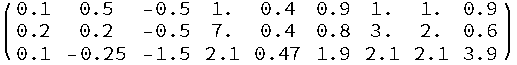
\includegraphics{refHmat.pdf}}}
\end{gather}
with $\psiCMat=\psiEpsMat=0, \,\,  \psi_z=I$.
I have chosen these coefficients so that 
the linear model has a unique stable solution and, since $H_1$ is full rank,
its row space will span the column space for all non zero values for $z_t \in \mathcal{R}^3$.\footnote{The flexibility in choosing $\linMod$ will 
become more important  later in the paper  where we must 
choose a  linear reference model in a context where we will have 
little guidance about what might make a good choice.}  

The solution for this system is

\begin{gather}
  B=
\vcenter{\hbox{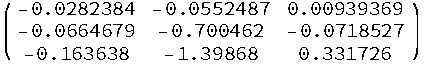
\includegraphics{refBmat.pdf}}}\\
\phiMat=
\vcenter{\hbox{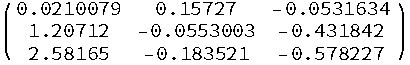
\includegraphics{refPhimat.pdf}}}\\
F=
\vcenter{\hbox{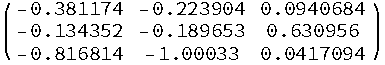
\includegraphics{refFmat.pdf}}}
\end{gather} 



It is straightforward to apply \ref{theSeries} to  the following three
bounded families of time series paths 
\begin{gather}
  x_{1,t}=\frac{\someNorm{x_{t-1}}}{{1+\someNorm{\theShock_{t}}}} D_\pi(t) \intertext{where $D_\pi(t)$ gives the t-th digit of $\pi$}
x_{2,t}=\frac{\someNorm{x_{t-1}}}{({1+\someNorm{\theShock_{t}}})^2} (-1)^t\\
ax_{3,t}=\theShock_t \intertext{and the $\theShock_t$ are a sequence of pseudo random draws from the uniform distributions $\mathcal{U}(-4,4)$ produced subsequent to the selection of a random seed.} randomseed(\someNorm{x_{t-1}}+\someNorm{\theShock_t})
\end{gather} 
The three panels in Figure \ref{arbpaths} display these three time series
generated  for a particular initial state vector and shock value.
 The first set of trajectories characterizes 
a function of the digits in the decimal representation of $\pi$. 
The second set of trajectories  oscillates between two values
determined by  a nonlinear function of the initial conditions, $x_{t-1}$ and the shock.
The third set of trajectories characterizes a sequence of uniformly distributed random numbers based on a seed determined by  a nonlinear function of  the initial conditions and the shock.
These paths were chosen to emphasize 
that continuity is not important for the existence of the series representation,
that the trajectories need not converge to a fixed point, and 
need not be produced by some linear rational expectations solution or by the
 iteration of a discrete-time map.
The spanning condition and the boundedness of the paths are  sufficient conditions for the existence 
of the series representation based on the 
linear reference model,$\linMod$.\footnote{Although potentially useful in some contexts,
this paper will not investigate representations for families of
unbounded, but slowly diverging  trajectories.}


\begin{figure}
  \centering
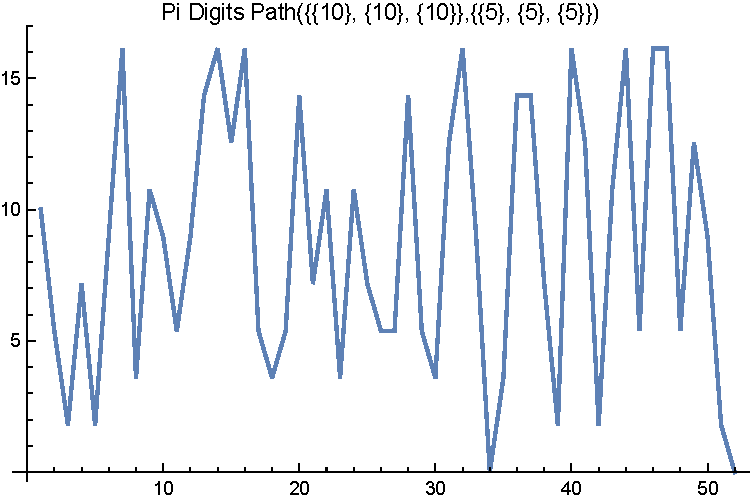
\includegraphics[width=2in]{piPath.pdf}
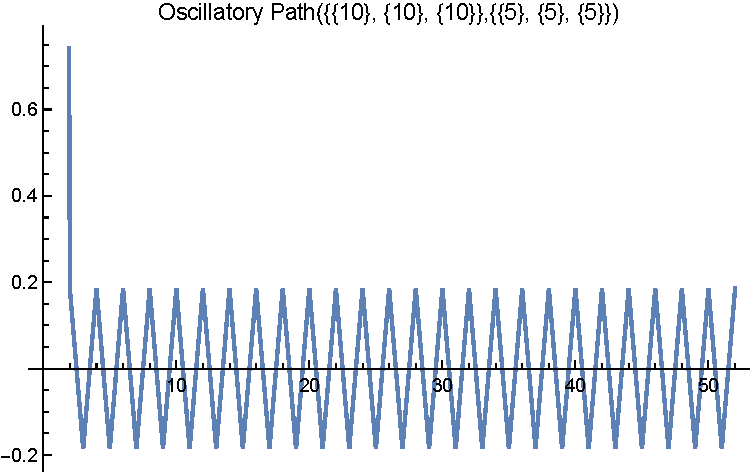
\includegraphics[width=2in]{oscillPath.pdf}
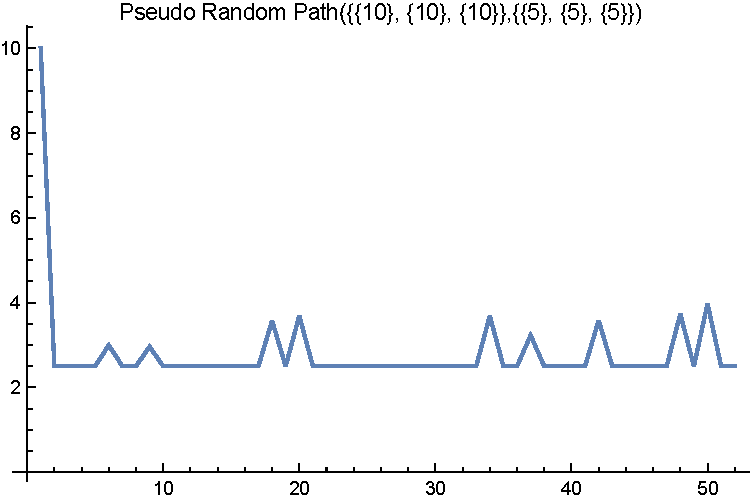
\includegraphics[width=2in]{pseudoPath.pdf}
  
  \caption{Arbitrary Bounded Time Series Paths}\label{arbpaths}
\end{figure}





Though unintuitive and perhaps lacking a compelling 
interpretation, the values for
$z_t$ exist,  provide  a series for the $x_t$  and are easy to compute.
One can apply the calculations for any given initial condition to produce
a z series exactly replicating any bounded set of trajectories.  
Consequently, these
numerical linear algebra calculations can easily transform a $z_t$ series into an $x_t$ series and vice versa.  Since this can be done for any path starting from any particular initial conditions, 
any discrete time invariant map that generates families of bounded paths has a series representation. Section \ref{sec:extToMaps} builds on this observation.





\subsection{Assessing $x_t$ Errors}
\label{sec:truncationerr}
The formula \ref{theSeries} 
computes the impact on the current state of fully anticipated future shocks.  It characterizes the impact exactly.  However one can contemplate the impact of at least two deviations from the exact calculation:
one could truncate a series of correct values of $z_t$ or
one might have imprecise values of $z_t$ along the path.

{\color{blue}
Should report units free Euler equation error for comparability to   Judd smolyak paper 2014.

Should compare and contrast to decision rule error.

Reproduce each of the combinations of param values as they did.

More interested in error in the decision rule than in model equation error.
}

\subsubsection{Truncation Error}


The series representation can compute the entire series exactly
if all the terms are included, but, it will at times be useful to exploit the fact that
the terms for state vectors closer 
to the initial time have the most important impact.
One could consider approximating  $\sVar_t$ by 
truncating the series  at a finite number of terms.
 	 \begin{gather}
 	 \sVarK_t \equiv B x_{t-1}+ \phiMat \psiEpsMat\theShock  + (I - F)^{-1} \phiMat \psiCMat + \sum_{s=0}^k F^s \phiMat z_{t}\label{theTruncSeries}
 \end{gather}
We can bound the  series approximation truncation errors:

    \begin{gather}
      \label{eq:1}
\sum_{s=k+1}^{\infty} F^s \phiMat \psi_z = (I -F)^{-1} F^{k+1}\phiMat \psi_z       \\
\infNorm{\xWarg-\xWargK} \le \infNorm{(I -F)^{-1} F^{k+1}\phiMat \psi_z} \left ( \infNorm{H_{-1} }+ \infNorm{H_{0} }+ \infNorm{H_{1} } \right )\infNorm{\overline{\mathcal{X}}}
    \end{gather}


 Figure \ref{figArbTrunc} shows
that this truncation error can be  a very conservative measure of the accuracy
of the truncated series.  The orange line represents the computed approximation of
the infinity norm of the difference between $x_t$ from the full series and a truncated series for different values of $k$, the length of the truncation.  The blue line shows the infinity norm of the actual difference between the $x_t$ computed using the full series and the value obtained using a truncated series.  The series requires only the first 20 terms to compute
the initial value of the state vector to high precision. 


\begin{figure}
  \centering


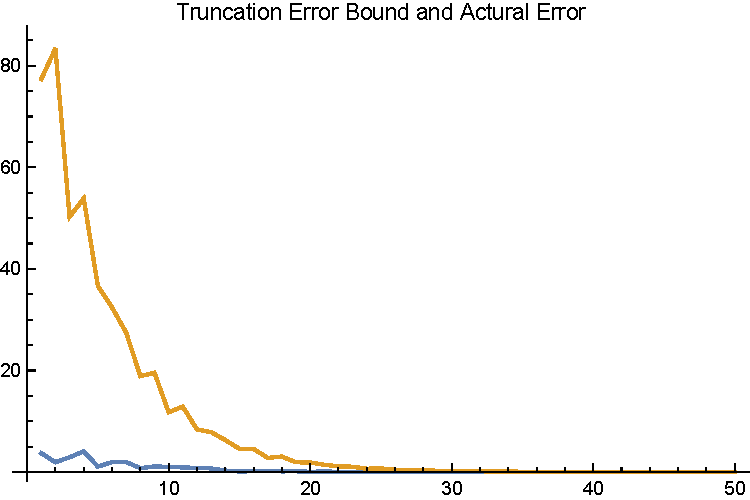
\includegraphics[width=3in]{arbTruncErr.pdf}  
  \caption{$x_t$ Error Approximation Versus Actual Error} \label{figArbTrunc}

\end{figure}

\subsubsection{Path Error}


We can assess the impact of perturbed values for $z_t$ by computing the maximum discrepancy,$\Delta z_t$, impacting the $z_t$ and applying the 
partial sum formula.
One can  approximate $\mathcal{X}_t$ using
 	 \begin{gather}
 	 \sVarK_t \equiv B x_{t-1}+ \phiMat \psiEpsMat\theShock  + (I - F)^{-1} \phiMat \psiCMat + \sum_{s=0}^\infty F^s \phiMat (z_{t}+\Delta z_{t})\label{theDeltaSeries}
 \end{gather}
Note, yet again, that for approximating $\xWarg$, the impact of  a given realization along the path declines for those realizations which are  more temporally distant.
However, we can conservatively bound the  series approximation  errors by using the largest possible $\Delta z_t$ in the formula:
    \begin{gather}
\infNorm{\xWarg-\xWargK} \le \infNorm{(I -F)^{-1} \phiMat \psi_z}  \infNorm{\Delta z_t } \label{pathErr}
    \end{gather}


\label{sec:pathnorm}

\clearpage
\section{Dynamic Stochastic Time Invariant Maps}
\label{sec:extToMaps}

Many dynamic stochastic models have solutions that 
fall in the class of bounded time invariant maps.
Consequently, if we take care (see Section \ref{sec:convenient}), we can apply the law of iterated expectations, 
to compute conditional expected solution paths 
forward from any initial value and realization of $\tArg$.\footnote{Economists have long used similar manipulation of
time series paths for dynamic models. 
Indeed, Potter constructs his generalized impulse response functions using
differences in conditional expectations paths \citep{Potter2000,Koop1996a}.
}
As a result, we can use the family of conditional expectations paths 
along with a contrived linear reference model to generate
a series representation for the model solutions  and
to approximate errors.

So long as the iterated trajectories of the conditional expectations paths are 
 bounded, the time invariant maps can 
be represented using the framework from section \ref{sec:newseries}.
The series representation will provide a linearly weighted sum of $z_t\tArg$ functions that give us an approximation for the model solutions.
This section presents a familiar RBC model as an example.\footnote{
Later, in order to handle models with regime switching and occasionally binding constraints, I will need to consider more complicated collections 
of equation systems with  Boolean gates. I will show how to apply the 
series formulation and to approximate the  errors for these models as well.}

%\subsection{Application of the Series Representation to Time Invariant Maps}




% Often these time invariant maps impose additional structure on the time 
% series they generate that allows us to use the series formula to
% develop bounds for the error in the solution.


\subsection{An RBC Example}
\label{sec:rbcaux}
  Consider the model described in  \citep{Maliar2005,Judd2014}\footnote{Here, I set their $\beta=1$ and 
do not discuss quasi-geometric discounting or time-inconsistency.}
 \begin{gather*}
   \max\left \{  u(c_t) + E_t \sum_{t=1}^\infty  \delta^{t}u(c_{t+1})\right \}\\
c_t + k_t= \theta_{t} f(k_{t-1})\\
f(k_t)= k_t^\alpha\\
u(c)=\frac{c^{1-\eta}-1}{1-\eta}
 \end{gather*}
The first order conditions for the model are

\begin{tcolorbox}[ams gather]
\frac{1}{c_t^{\eta}}=\delta \left ( \alpha k_{t}^{\alpha-1} E_t \left (\frac{\theta_{t+1}}{c_{t+1}^\eta} \right )+ (1-d)E_t\left (\frac{1}{c_{t+1}^\eta} \right ) \right )\\
c_t + k_t=(1-d)k_{t-1}\theta_{t}k_{t-1}^\alpha \\
 \theta_t =\theta_{t-1}^\rho e^{\theShock_t}\label{rbcSys}
 \end{tcolorbox}
\label{sec:rbcexample}

For comparison with results reported in \citep{Judd2014} it will be useful
to recast the first equation in unit free form:

\begin{gather*}
\delta c_t^{\eta}\left ( \alpha k_{t}^{\alpha-1} E_t \left (\frac{\theta_{t+1}}{c_{t+1}^\eta} \right )+ (1-d)E_t\left (\frac{1}{c_{t+1}^\eta} \right ) \right ) -1\\
\end{gather*}

It is well known that when $\eta=1$, we have a closed form solution \citep{lettau03}:
\begin{gather}
x_t(\xtmEpsArg)\equiv    \DR(\xtmEpsArg)\equiv
   \begin{bmatrix}
     c_t(\xtmEpsArg)\\k_t(\xtmEpsArg)\\ \theta_t(\xtmEpsArg)
   \end{bmatrix}=
   \begin{bmatrix}
(1-\alpha \delta) \theta_{t} k_{t-1}^\alpha\\
  \alpha \delta \theta_{t} k_{t-1}^\alpha.\label{soln}\\
\theta_{t-1}^\rho e^{\theShock_t}.
   \end{bmatrix}
\end{gather}
For mean zero iid $\theShock_t$ we can easily 
compute the conditional expectation of the model variables for any given $\theta_{t+k},k_{t+k}$
\begin{gather*}
  \DRCE(x_{t+k+1})\equiv
  \begin{bmatrix}
  E_t(c_{t+k+1}|\theta_{t+k},k_{t+k})\\
  E_t(k_{t+k+1}|\theta_{t+k},k_{t+k})\\
  E_t(\theta_{t+k+1}|\theta_{t+k},k_{t+k})
  \end{bmatrix}=
  \begin{bmatrix}
(1-\alpha\delta)k_{t+k}^\alpha e^{\frac{\sigma^2}{2}}\theta_{t+k}^\rho\\
\alpha\delta k_{t+k}^\alpha e^{\frac{\sigma^2}{2}}\theta_{t+k}^\rho\\
e^{\frac{\sigma^2}{2}}\theta_{t+k}^\rho
  \end{bmatrix}
\end{gather*}


For any given values of $k_{t-1},\theta_{t-1}, \theShock_t$, the model decision rule, ($\DR$), and decision rule conditional expectation, ($\DRCE$), can generate a conditional expectations path forward from  any given initial $\tArg$:
\begin{gather*}
  \sVar_t(\xtmEpsArg)=\DR(\xtmEpsArg)\\
  \sVar_{t+k+1}(\xtmEpsArg)=\DRCE(\sVar_{t+k}(\xtmEpsArg))
\end{gather*}
and corresponding paths for $\{(z_{1t}\tArg, z_{2t}\tArg, z_{3t}\tArg),\ldots\}$
\begin{gather*}
  z_{t+k} \equiv H_{-1} \sVar_{t+k-1} +  H_0 \sVar_{t+k} +  H_1 \sVar_{t+K+1} 
\end{gather*}
Formula \refeq{theSeries} requires that
\begin{gather*}
%   \begin{bmatrix}
% c_t(k_{t-1},\theta_{t-1}, \theShock_t)\\
% k_t(k_{t-1},\theta_{t-1}, \theShock_t)\\
% \theta_t(k_{t-1},\theta_{t-1}, \theShock_t)
%   \end{bmatrix} \rightarrow
%   \begin{bmatrix}
%   z_{1t}(k_{t-1},\theta_{t-1}, \theShock_t)\\
%   z_{2t}(k_{t-1},\theta_{t-1}, \theShock_t)\\
%   z_{3t}(k_{t-1},\theta_{t-1}, \theShock_t) 
%   \end{bmatrix}\equiv z(k_{t-1},\theta_{t-1}, \theShock_t)\intertext{where}
%   \begin{bmatrix}
% c_t(k_{t-1},\theta_{t-1}, \theShock_t)\\
% k_t(k_{t-1},\theta_{t-1}, \theShock_t)\\
% \theta_t(k_{t-1},\theta_{t-1}, \theShock_t)
%   \end{bmatrix}  =
\sVar(\xtmEpsArg)=
B   \begin{bmatrix}
c_{t-1}\\
k_{t-1}\\
\theta_{t-1}
  \end{bmatrix}  + \phiMat \psiEpsMat\theShock_t + (I - F)^{-1} \phiMat \psiCMat + \sum_{\sumIdx=0}^\infty F^s \phiMat z_{t+\sumIdx}(k_{t-1},\theta_{t-1}, \theShock_t) 
\end{gather*}
% \footnote{
% We need not  make these adjustments for the steady state,
% but doing so economizes on the number of terms 
% required for a given level of approximation
% accuracy.}

For example, using $\eta=d=1$ and the following parameter values and using the arbitrary linear reference model \eqref{linRef} we can generate a series representation for the model solutions.

% \begin{gather}\label{rbcparams}
% \vcenter{\hbox{\includegraphics{RBCParamSubs.pdf}}} \,\, \text{ we have } \,\,
%   \begin{bmatrix}
%     c_{ss}\\k_{ss} \\ \theta_{ss} 
%   \end{bmatrix}=
% \left [ \vcenter{\hbox{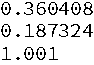
\includegraphics{RBCSSVal.pdf}}}\right ]
% \end{gather}



\begin{gather}\label{theInits}
  \begin{bmatrix}
 k_{t-1}\\\theta_{t-1}\\\theShock_t 
  \end{bmatrix}=
\left [ \vcenter{\hbox{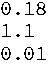
\includegraphics{anXEps.pdf}}}\right ]
\end{gather}


\begin{figure}
  \centering
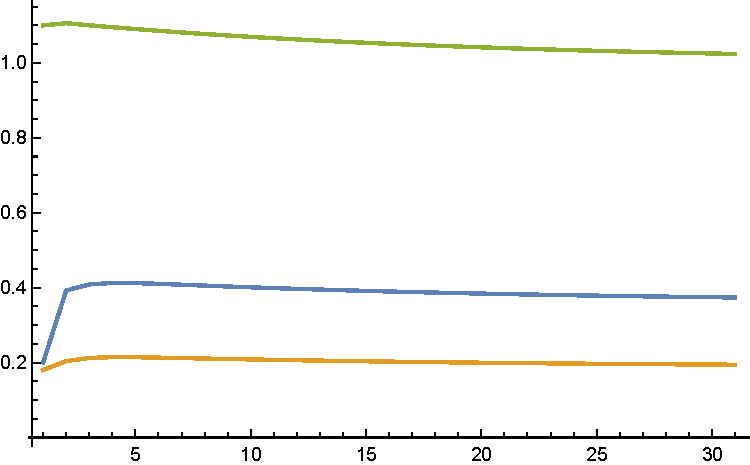
\includegraphics[width=3.0in]{simprbcvals.pdf}  %\hspace{.75in}
%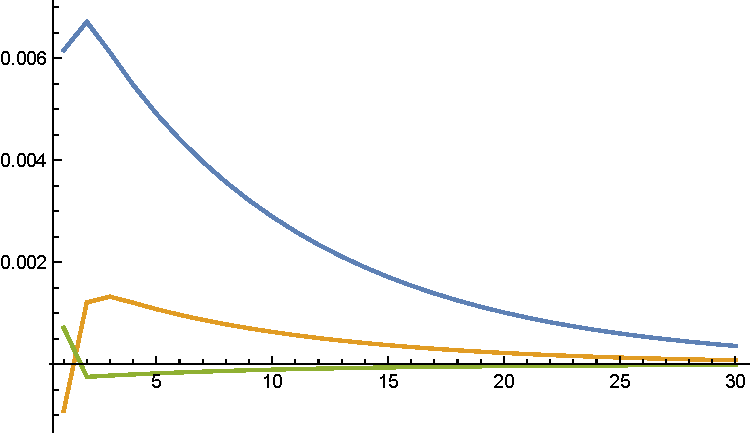
\includegraphics[width=3.0in]{simprbczvals.pdf}  
  \caption{model variable values}
  \label{rbcpaths}
\end{figure}

Figure \refeq{rbcpaths} shows, from top to bottom, the paths of $\theta_t, c_t, \text{ and } k_t$ from the initial values given in Equation \refeq{theInits}. 
%The orange line corresponds to $z_{1t}\tArg$,the blue line corresponds to $z_{2t}\tArg$ and the green line corresponds to $z_{3t}\tArg$.%\footnote{For now we focus on the times series paths, $z_t(x_{t-1},\theShock_t)$ for given $(x_{t-1},\theShock_t)$.  Later we will exploit the information available from explicit investigation of the variation in  $z_t(x_{t-1},\theShock_t)$ with $(x_{t-1},\theShock_t)$ to improve solution accuracy and robustness.}
By including enough terms we can compute the solution for $x_t$ 
exactly.
Figure \ref{rbcTrunc} shows the impact that truncating the series has 
on approximation of the time t values of the state variables.   The approximated magnitude for the error, $B_n$, shown in red 
 is again very pessimistic compared to the actual error, $Z_n=\infNorm{x_t-x_t^\star}$, shown in blue.
With enough terms, even using an ``almost'' arbitrarily chosen linear model,  the series approximation provides a machine precision accurate value for the time t state vector. 

\begin{figure}
  \centering
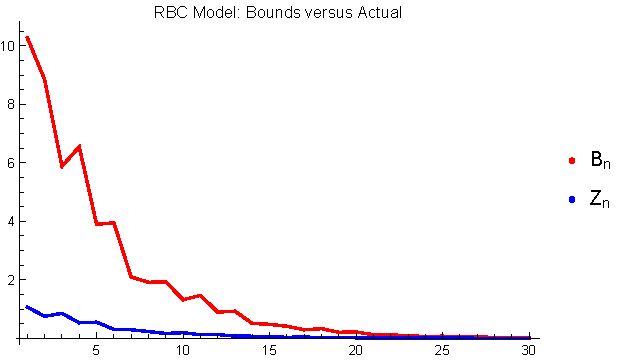
\includegraphics[width=2.7in]{simpArbBoundsVActual.pdf}  
  \caption{RBC Known Solution: Truncation Approximate Error  Versus Actual: ``Almost Arbitrary'' Linear Reference Model}
  \label{rbcTrunc}
\end{figure}
\begin{figure}
  \centering
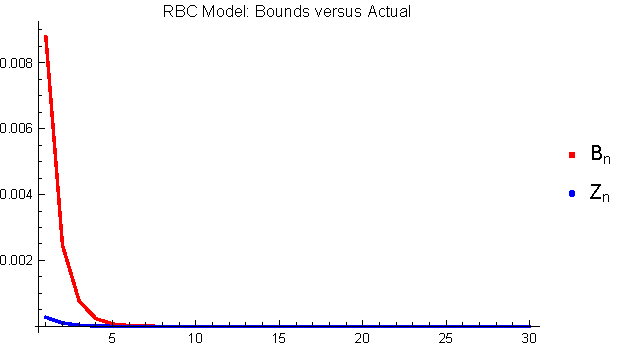
\includegraphics[width=2.7in]{simpBoundsVActual.pdf}  
  \caption{RBC Known Solution: Truncation Approximate Error Versus Actual: Stochastic Steady State Linearization Linear Reference Model}
  \label{rbcTruncSimp}
\end{figure}



Figure \ref{rbcTruncSimp} shows that using a 
linearization that better tracks the 
nonlinear model paths, improves the approximation $Z_n$, shown in blue  and the approximate error  $B_n$ shown in red.
Using the linearization of the RBC model around the ergodic mean produces a tighter but still  pessimistic bound on the errors for the initial state vector.
Again, the first few terms make most of the difference in approximating the value of the state variables.


\subsection{A Model Specification Constraint}
\label{sec:convenient}



For convenience of notation in what follows, 
I will focus on models built up from components of the form
\begin{gather}
  h_i(x_{t-1},x_{t},x_{t+1},\theShock_t)=h^{det}_{io}(x_{t-1},x_{t},\theShock_t)+\sum_{j=1}^{p_i} [h^{det}_{ij}(x_{t-1},x_{t},\theShock_t)h^{nondet}_{ij}(x_{t+1})]=0
\end{gather}
This is a very broad class of models including most widely used
macroeconomics models.  This constraint will make it easier to write
down and manipulate the conditional expectations expressions in the
description of the algorithms in subsequent sections.
For example, the Euler equations for the  neoclassical growth  model 
\label{sec:simple-rbc-model-ext} can be written as
\begin{gather}
h_{10^{det}}(\cdot)=\frac{1}{c_t^\eta},\,\,
h_{11}^{det}()=\alpha \delta k_{t}^{\alpha-1} ,\,\,
h_{11}^{nondet}(\cdot)=E_t \left (\frac{\theta_{t+1}}{c_{t+1}^\eta} \right )\\
h_{20}^{det}(\cdot)=c_t + k_t-\theta_tk_{t-1}^\alpha,\,\,
h_{21}^{det}(\cdot)=0\\
h_{30}^{det}(\cdot)=\ln \theta_t -(\rho \ln \theta_{t-1} + \theShock_t),\,\,
h_{31}^{det}(\cdot)=0
\end{gather}
Since we   need to compute 
the conditional expectation of nonlinear expressions,  
this setup will make it possible for us to use auxiliary
variables to correctly compute the required expected values.
\label{simpRBCExample}
We will be working with models where expectations are computed at time t, with  $\theShock_t$  known. 
We can construct a linear reference model for the modified RBC system
by  augmenting the RBC model with the equation 
\begin{tcolorbox}[ams gather]
  \rcpC_{1,t}=\frac{\theta_t}{c_t},  \rcpC_{2,t}=\frac{1}{c_t},
\end{tcolorbox}
\noindent
substituting $\rcpC_{1,t+1}$ for $\frac{\theta_{t+1}}{c_{t+1}}$ and
$\rcpC_{2,t+1}$ for $\frac{1}{c_{t+1}}$
in the first equation and 
 linearizing the RBC model about the ergodic mean.

This leads to:

%    \begin{gather}
%  H_{-1}=\vcenter{\hbox{\includegraphics{rbcExampleOctoberHM.pdf}}} \\
% H_{0}=\vcenter{\hbox{\includegraphics{rbcExampleOctoberHZ.pdf}}} \label{rbcLinSys}\\  
% H_{1}=\vcenter{\hbox{\includegraphics{rbcExampleOctoberHP.pdf}}} \intertext{with}
%  \psiEpsMat= \begin{bmatrix}
%    0\\0\\0\\0\\1
%  \end{bmatrix}, \psi_z=I_5
%  \end{gather}

These coefficients  produce a unique stable linear solution.\footnote{$H_{1}$  has only one non-zero term here since $d=1$.}

% \begin{gather}
%   B=
% \vcenter{\hbox{\includegraphics{rbcExampleOctoberB.pdf}}},
% \phiMat=
% \vcenter{\hbox{\includegraphics{rbcExampleOctoberPhi.pdf}}}\\
% F=
% \vcenter{\hbox{\includegraphics{rbcExampleOctoberF.pdf}}}\\
% \psiCMat=\vcenter{\hbox{\includegraphics{rbcExampleOctoberPsiC.pdf}}}
% \end{gather}
Recomputing the truncation errors with the expanded model produces nearly identical results for  variable approximation errors.


\clearpage
\section{Approximating Model Solution Errors}
\label{sec:solnerrorbounds}


This section shows how to use the model equation errors  to construct an 
approximate error for the components of any proposed
model decision rule solution.   Here I provide
a formula for the approximate error that does not require statistical inference.\footnote{This work contrasts with the analysis provided in
 \citep{judd2017lower,peralta-alva14,santos2005accuracy,Santos2000accuracy}. 
Their approaches identify Euler Equation Errors, but use statistical techniques to estimate the impact of these errors on solution accuracy.  Here I provide
a formula for the approximate error that does not require statistical inference.}



\subsection{Approximating a Global Decision Rule Error Bound}
\label{sec:an-error-bound}



%\subsection{An Error Approximation Formula}
\label{sec:errorformula}

Consider a bounded region, $\bndRgn$, that contains all iterated conditional expectations paths.
  By bounding the largest deviation in the paths for the $\Delta z_t^p$, we can bound the largest deviation in a proposed model decision rule solution from the exact solution. 



Given an exact solution $x^\star_t=g^\star(x_{t-1},\theShock_t)$ define the conditional expectations function,
  \begin{gather}
G^\star(x)\equiv\expct{g^\star(x,\theShock)} \intertext{then with}
E_tx^\star_{t+1}=G^\star(g^\star(x_{t-1},\theShock_t)) \intertext{we have}
    \label{eq:2}
\eqnFunc(x^\star_{t-1},x^\star_t,E_tx^\star_{t+1},\theShock_t)=0  \,\, \forall  (x_{t-1},\theShock_t)\\ 
   x^\star_t(x_{t-1},\theShock_t) \in{R^L}\,\,\twoNorm{x^\star_t(x_{t-1},\theShock_t)}  \le \overline{\mathcal{X}}\,\,\forall t\ > 0
  \end{gather}

Now consider a proposed model decision rule solution for the model,
 $x^p_t=g^p(x_{t-1},\theShock_t)$ define
$G^p(x)\equiv\expct{g^p(x,\theShock)}$  so that 
  \begin{gather*}
E_tx_{t+1}=G^p(g^p(x_{t-1},\theShock_t))\\
\mathbf{e}_t^p(x_{t-1},\theShock)\equiv
\eqnFunc(x_{t-1},x^p_t,E_tx^p_{t+1},\theShock_t)
\end{gather*}


    \begin{gather*}
	\infNorm{ x^\star_{t}(x_{t-1},\theShock) -	 x^p_{t}(x_{t-1},\theShock)} \le
\max_{\{x_{-},\theShock\}} \twoNorm{(I-F)^{-1} \phiMat \eqnFunc(x_{-},g^p(x_{-},\theShock),G^p(g^p(x_{-},\theShock)),\theShock) }\intertext{which can be approximated by}
    \max_{x_{t-1},\theShock_t} (\phiMat \mathbf{e}_t^p(x_{t-1},\theShock))^2
  \end{gather*}

For proof see Appendix \ref{sec:error-bound-formula}.  

\subsection{Approximating Local Decision Rule Errors}
\label{sec:decis-rule-comp}

Given a proposed decision rule  solution define 
the error in $x_t$ at $\tArg$

\begin{gather*}
\mathbf{e}\tArg\equiv \sVar^\star\tArg-\sVar^p\tArg\intertext{compute the conditional expectations functions for the decision rule and use them to generate a path to use with a linear reference model $\linMod  \equiv \linModMats$  in \ref{theSeries} to approximate  $\mathbf{e}$.} 
\XVar^p(x)\equiv \expct{\sVar^p(x,\theShock)}.
\end{gather*}
\begin{gather*}
 x_{t+k+1}=\XVar^p(x_{t+k})\,\,k=1,\ldots,K
\end{gather*}

\begin{gather*}
 \intertext{We can define functions $\zpVar_t$ by}
\zpVar_t\equiv
\eqnFunc(x_{t-1},x_t,x_{t+1},\theShock_t)\\
\zpVar_{t+k}\equiv
\eqnFunc(x_{t+k-1},x_{t+k},x_{t+k+1},0)\\
\hat{\mathbf{e}}\tArg\equiv \sum_{\sumIdx=0}^K F^s \phiMat \zpVar_{t+\nu}\\
\end{gather*}

\subsection{Assessing the Error Approximation}
\label{sec:assess-error-appr}


This section reports on the results of an experiment evaluating how well the 
formula performs.  
I compute the known decision rule for the RBC model with parameters
$\{\alpha=0.36,\delta=0.95,\eta=1,\rho=0.95,\sigma=0.01\}$.  I consider this
the fixed ``true'' model.

I generate  10 other settings for the model parameters by choosing
parameters from the ranges:
\begin{gather*}
 0.20 <\alpha<0.40,\,\,0.85<\delta<0.99,\,\,0.85<\rho<0.99,\,\,0.005<\sigma<0.015
\end{gather*}
producing the following 10 model specifications:


\vspace{.2in}



   \begin{tabular}{|c|c|c|c|c|}
\hline
\multicolumn{1}{|c|}{$\alpha$}&
\multicolumn{1}{|c|}{$\delta$}&
\multicolumn{1}{|c|}{$\eta$}&
\multicolumn{1}{|c|}{$\rho$}&
\multicolumn{1}{|c|}{$\sigma$}\\
\hline
                   0.35 & 0.92875 & 1. & 0.957188 & 0.00875 \\
\hline
                   0.275 & 0.9725 & 1. & 0.906875 & 0.01375 \\
\hline
                   0.375 & 0.8675 & 1. & 0.924375 & 0.01125 \\
\hline
                   0.225 & 0.94625 & 1. & 0.891563 & 0.00625 \\
\hline
                   0.325 & 0.91125 & 1. & 0.944063 & 0.006875 \\
\hline
                   0.2625 & 0.922187 & 1. & 0.98125 & 0.011875 \\
\hline
                   0.3625 & 0.887187 & 1. & 0.85875 & 0.014375 \\
\hline
                   0.2125 & 0.965938 & 1. & 0.965938 & 0.009375 \\
\hline
                   0.3125 & 0.860938 & 1. & 0.878438 & 0.008125 \\
\hline
                   0.2375 & 0.904688 & 1. & 0.933125 & 0.013125 \\
\hline
                  \end{tabular}


\vspace{.2in}



I linearized each of the ten models at their respective stochastic steady
states producing 10 linear reference models $\linMod_i$ and 10 decision rules
based on the linearization. 
As a result I have $100=10 \times 10$ combinations of (inaccurate by design ) decision rule functions
 and
linear reference models to use in the error formula experiments.


I generate 30 representative points, $(k_{i,t-1},\theta_{i,t-1},\theShock_{i,t})$, from the ergodic set for the fixed true reference model
using the Niederreiter quasi-random algorithm.
For each of the 100 pairings of decision rule and linear reference model,
I compute the error approximation at each of the 30 representative points
and regress the actual error, computed using the known analytic solution, and the predicted error from the error formula:
\begin{gather*}
  \mathbf{e_i}=\alpha + \beta   \hat{\mathbf{e_i}} +u_i
\end{gather*}
Although the true model and the true decision rule stays 
fixed in the experiment, the
  proposed decision rules and the linear reference models both change.

Figures \ref{fig:forc} and \ref{fig:fork}  present the 100 $R^2$'s and estimated variance, $\hat{\sigma}^2$ and Figures \ref{fig:forcn} and \ref{fig:forkn} presents the 100 resulting regression coefficients, $ (\alpha,\beta)$ for a variety of values for $K$, of number of terms in the 
error formula, ( $K=0, 1, 10, 30$)\footnote{I don't display results for $\theta_t$ because the formula predicts the error 
in $\theta_t$ perfectly since it is determined by a backward looking equation.}
( The regressions with $K=0$ correspond to the maximand of the
global error formula. ) The figures show that
the formula does a good job of predicting the error produced by the 
inaccurate decision rule functions.
Even with $K=0$, using only one term in the error formula,
 still provides 
useful information about the magnitude of the discrepancy between the 
proposed decision rules values and true values.  The $R^2$ values are all above 60 percent and are often near one.  The $\beta$ coefficients are generally  close to one and the 
constant tends to be close to zero. {\color{blue} Increasing $k$ initially increases accuracy,
but utimately the inaccuracy of the conditional expectation path reduces
the accuracy of the estimates with many terms.}



\begin{figure}
  \centering
  %\includegraphics[width=3.0in]{cRegRSQ10x0.pdf}
   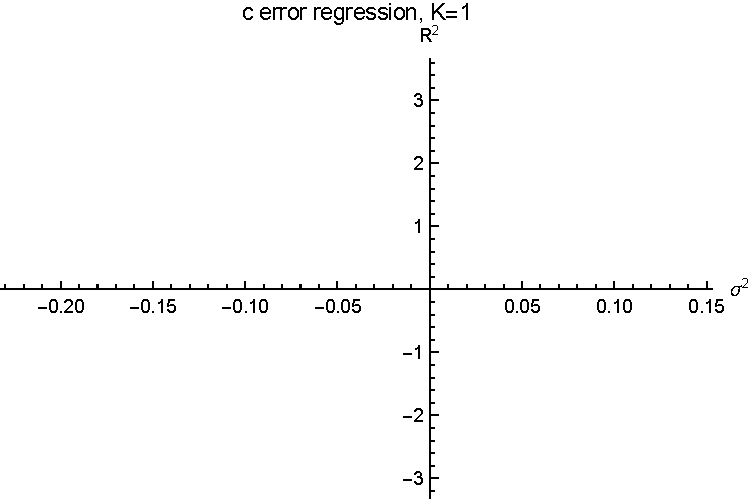
\includegraphics[width=3.0in]{cRegRSQ10x1.pdf}
  % \includegraphics[width=3.0in]{cRegRSQ10x10.pdf}
  % \includegraphics[width=3.0in]{cRegRSQ10x30.pdf}
  \caption{$c_t\, (\hat{\sigma^2},R^2)$ \label{fig:forc}}
  
\end{figure}


\begin{figure}
  \centering
  % \includegraphics[width=3.0in]{kRegRSQ10x0.pdf}
  % \includegraphics[width=3.0in]{kRegRSQ10x1.pdf}
  % \includegraphics[width=3.0in]{kRegRSQ10x10.pdf}
  % \includegraphics[width=3.0in]{kRegRSQ10x30.pdf}
  \caption{$k_t\, (\hat{\sigma^2},R^2) $   \label{fig:fork} }

\end{figure}



\begin{figure}
  \centering
  % \includegraphics[width=3.0in]{cReg10x0.pdf}
  % 
\includegraphics[width=3.0in]{cReg10x1.pdf}
  % \includegraphics[width=3.0in]{cReg10x10.pdf}
  % \includegraphics[width=3.0in]{cReg10x30.pdf}
  \caption{$c_t\, (\alpha,\beta)$ \label{fig:forcn}}
  
\end{figure}


\begin{figure}
  \centering
  % \includegraphics[width=3.0in]{kReg10x0.pdf}
  % \includegraphics[width=3.0in]{kReg10x1.pdf}
  % \includegraphics[width=3.0in]{kReg10x10.pdf}
  % \includegraphics[width=3.0in]{kReg10x30.pdf}
  \caption{$k_t\, (\alpha,\beta) $   \label{fig:forkn} }

\end{figure}






\clearpage
\section{Improving Proposed  Solutions}
\label{sec:algoforsoln}


\subsection{Some Practical Considerations for Applying the Series Formula}
\label{sec:practicalformula}

% The framework provides a new way to bound the error one can expect from
% employing a given proposed model solution and leads, in Section \ref{sec:algoforsoln},, to an
% algorithm with  components similar to parameterized expectations that
% one can use to improve proposed solutions. In that section, the
% series representation makes
% it possible to organize the calculation around computing a deterministic
% problem at time t given a proposed solution.  The deterministic solution
% can accommodate inequality constraints or alternative regimes to produce a
% solution for each set of initial conditions.  One can typically arrange,
% perhaps by adding auxiliary variables, to produce a ``decision rule''
% that one can use to correctly precompute a deterministic conditional
% expectation function that can be iterated forward and serves to
% improve upon the original proposed solution.
% Time invariant stochastic functions 
% lead naturally to an associated family of deterministic maps
% which can be conveniently represented by the series representation.


% The paper studies a very general class of models whose 
% solutions are characterized by $\eqnFuncSys$, an
%  exhaustive and mutually exclusive set 
% of   triples, $\eqnFuncSysI{i}\equiv\{\eqnFunc_i,\preGate_i,\postGate_i\}$, with model equations,  $\eqnFunc_i$,  and Boolean valued gates, $\preGate_i$, $\postGate_i$. 
% that together determine a unique  solution  $x_t\tArg$
%\begin{gather}
%\intertext{ where, each }
%\eqnFuncSysI{i}\equiv \eqnFuncSysIExpl{i} \label{eqnGates}
%\end{gather}

{\color{blue}
For robustness, one needs to ``re-route'' trajectories that stray from the
ergodic set during the search for a solution.  These proposed decision rule
solutions 
cab explode and become unbounded.  They pollute the calculations in the
error formula and in the augmented system.

Probably need homotopy to get larg $\eta$ in RBC, but the extra constraints
facilitate this.

Check that explosive conditional expectation can't simulate bounded.
Related to pruning?

Use  JEDC 2014 RBC 


My method handles Multiple expectational equations  impact on decision rules.
}


I assume that all models of interest can be characterized by
 a finite number of equations systems.
I will require that, for any 
 given $(x_{t-1},\theShock_t)$,  this collection of 
equation systems  produces a unique solution for $x_t$.  
This formulation will allow us to apply the technique to models with
occasionally binding  constraints and models with regime switching.
I will only consider time invariant model solutions $x_t=\xWarg$.  Given a decision rule $\xWarg$, denote its conditional expectation $\XVar(x_{t-1})\equiv \expct{\xWarg}$.
Using the convention described in section \ref{sec:convenient}, 
 I will include 
enough auxiliary variables so that I can correctly compute expected values
for model variables by applying the law of iterated 
expectations.

It will be convenient for describing the algorithms to
write the models in the form
\begin{gather}
\eqnFuncSys \intertext{ where, each }
\eqnFuncSysI{i}\equiv \eqnFuncSysIExpl{i} \label{eqnGates}
\end{gather}
 represents a set of model equations, $\eqnFunc_i$,  with Boolean valued gate functions, $\preGate_i, \postGate_i$. 
In the algorithm's implementation, the $\preGate_i$ will be a 
Boolean pre-condition  function and 
the $\postGate_i$ will be a 
Boolean post-condition  functions for a given equation system. If some $\preGate_i$ is false, then there is no need to try to solve model $i$. 
If $\postGate_i(x_t\tArg)$ is false, the system has produced an unacceptable solution which should be ignored.
I suggest organizing equations using pre and post conditions as
this can help with parallelizing a solution regardless of whether or not
one uses my series representation. The
$\lastGate$ will be a function for choosing among the 
candidate $x_t\tArg$ values.
The function $\lastGate$ uses the truth values from the $(\preGate_.,\postGate_.)$ and the possible values of the state variables to select one and only one $x_t$.  Thus, we will have an equation system and  corresponding gatekeeper 
logical expressions 
indicating which equation system is in force for producing the unique
solution for a given $\tArg$.



 Examples of such systems include the simple RBC model from Section
\ref{simpRBCExample}.
Other examples include  models with 
occasionally binding constraints where solutions 
exhibit complementary slackness conditions, or models with 
regime switching.   See Section \ref{sec:occbind} for a model with
occasionally binding constraints and
Section \ref{sec:ressw} for an example 
of a specification for regime switching.






\subsection{How My Approach Differs From the Usual Approach}
\label{sec:walkthrough}


It may be worthwhile at this point
to briefly compare and contrast the approach I propose here with 
what is typically done when using projection methods 
for solving dynamic stochastic models.
As with the standard approach, I characterize the solutions using a linearly
weighted sums of orthogonal polynomials and solve the model equations
at predetermined collocation points. However, in this new algorithm, I 
augment the model Euler equations with equations based on \refeq{theSeries}
  linking the conditional expectations for future values in
the proposed decision rule solution with the
time t value of the model variables.  As a result, the algorithm determines
linearly weighted polynomials characterizing the 
trajectories for the usual
variables $x_t(x_{t-1},\theShock_t)$ as well as new  $z_t(x_{t-1},\theShock_t)$ variables.  These new constraints 
help keep proposed solutions bounded during the solution iterations 
thus improving algorithm reliability and accuracy.




% \begin{itemize}
% \item show describe $z_t(x_{t-1},\theShock_t)$ for RBC
% \item start linear.  check error bounds, if adequate done
% \item traditional iteration ignores the path constraints on initial solution leading to larger errors on $\bndRgn^p$
% \item It's a good idea to compute easy approximation using just the linear model one ieration to get an approximation for the ergodic set
% \item PEA moving bounds  \citep{maliarmovingbounds}
% \item them simulate and make the Maliar SVD transformation
% \item then iterate on the ergodic set till it settles down
% \item in this way can avoid solutions which are explosive when iterated 
% \item need to see if this works when honoring complimentary slackness
% \item not related to z transform. probably should change z's
% \end{itemize}


\subsection{Algorithm Overview}

% \subsubsection{Approximating an Unknown Solution: $U(c) \ne Log(c)$ }
% \label{sec:unknown-solutions}

Since I closely follow the techniques outlined in  \citep{Judd2013,Judd2014}. 
As a result, much of what must be done to use this  algorithm is 
the same as for the usual approach.
One must specify an initial guess for decision rule $\xWargK$ and obtain conditional expectations functions.
I use the an-isotropic Smolyak Lagrange interpolation with adaptive domain.
I precompute all of the conditional expectations for the integrals as outlined in  \citep{NBERw17418} so that the time t computations \ref{eqnGates} are all 
deterministic.




There are a number of new steps. 
One must  specify a linear reference model.
  One must choose a value for
$K$ the number of terms in the series representation.  There are trade-offs.
Small $k$  means more truncation error. 
Large $k$ corresponds to more accuracy when the decision rule is accurate but
is computationally more expensive. The initial guess is 
typically some distance away from the solution.   Consequently the
terms in the series will be incorrect.  The Smolyak grid adds more error to
the calculation.  If there are many grid points it is more likely that 
increasing the K can improve the quality of the solution.  If the grid is
too sparse, increasing K will likely be less useful. 

{\color{blue}
More research needed on selecting $k$.

Should always iterate forward from evaluation points to check stability.

}






\subsubsection{Single Equation System Case}

For now, consider a single model equation system case with no Boolean gates. A description 
of the actual, multi-system implementation follows.   We seek 
\begin{gather*}
\eqnFunc(x_{t-1},\sVar^\star\tArg,\XVar^\star(\sVar^\star\tArg),\theShock_t)=0\,\,\forall \tArg.  \intertext{Given a proposed decision rule model solution}
 x_t=\sVar^p\tArg\intertext{ compute}
\XVar^p(x_{t-1})\equiv \expct{\sVar^p\tArg}.
\end{gather*}
We will use a linear reference model $\linMod  \equiv \linModMats$ 
to construct a series of $\zpVar$ functions that help 
improve the accuracy of the proposed solution.





\begin{gather*}
 \intertext{We can define functions $\zpVar,\ZpVar$ by}
\zpWarg\equiv H
\begin{bmatrix}
x_{t-1}\\ \xpWarg\\ \XpVar(\xWarg)
\end{bmatrix}+\phiMat_\theShock \theShock_t+\phiMat_c\\
\ZpVar(x_{t-1})\equiv \expct{\zpWarg}
\end{gather*}
 \begin{itemize}
\item  {\color{blue}Algorithm loop begins here.} Define conditional expectations paths for $x_t, z_t$ 
 \begin{gather*}
 x_{t+k+1}=\XVar(x_{t+k}),\,\,\,z_{t+k+1}=\ZVar(x_{t+k})\,\,\,\,  \forall k\ge 0      \end{gather*}
% \item
% it will be useful to construct an augmented decision rule,
% $\ADR\tArg\equiv
%   \begin{bmatrix}
%     x^p\tArg\\z^p\tArg
%   \end{bmatrix}$, initially $z^p\tArg=0$
   \end{itemize}

{Using the $\zpWarg$ Series}
{\small
  \begin{itemize}
  \item We get expressions for $x_t,\,\, \expct x_{t+1}$ consistent with $\linMod$ and the conditional expectations path
   \begin{gather*}
     \mathcal{X}_{t} =B x_{t-1}+ \phiMat \psiEpsMat\theShock + (I - F)^{-1} \phiMat \psiCMat + \sum_{\sumIdx=0}^\infty F^s \phiMat \ZVar(x_{t+\nu})\\
	\expct{ \mathcal{X}_{t+1}} =B \mathcal{X}_{t}  + (I - F)^{-1} \phiMat \psiCMat+ \sum_{\sumIdx =0}^\infty F^{\sumIdx-1} \phiMat \ZVar(x_{t+\nu}) \,\,\,\,\,\forall t,k \ge  0
\end{gather*}
\item Use the model equations, $\eqnFunc(x_{t-1},x_t,\expct{x_{t+1}},\theShock)=0$ and $x_t\tArg=\mathcal{X}_t\tArg$\\ to determine $\xppWarg, \zppWarg$
\item $\xpWarg=\xppWarg, \zpWarg=\zppWarg$ -- {\color{blue}Repeat loop.}
  \end{itemize}
}

\subsubsection{Multiple Equation System Case}


An outline of the current Mathematica implementation of the algorithm follows.
Table \ref{algnotation} provides notation.
\begin{table}[h]
  \centering
\begin{description}
\item[$\linMod\equiv \linModMats$] The linear reference model
\item[$ \sVar^{p}\tArg$] The proposed decision rule  $x_t$ components
\item[$ \zVar^{p}\tArg$]The proposed decision rule  $z_t$ components
\item[$ \XVar^p\tNo$] The proposed decision rule conditional expectations  $x_t$ components
\item[$ \ZVar^p\tNo$] The proposed decision rule their conditional expectations  $z_t$ components
\item[$ \kappa$] One less than the number of terms in series representation$(\kappa>=0)$
\item[$\smolSpec$] Smolyak an-isotropic grid polynomials $(\aSmolPoly{1},\ldots,\aSmolPoly{N})$ and their conditional expectations $(\aSmolPolyCE{1},\ldots,\aSmolPolyCE{N})$
\item[$\mathbb{T}$] Model evaluation points Neidereiter sequence in the model variable ergodic region.
\item[$ \xzFunc$]  $\{\sVar\tArg,\zVar\tArg\}$ collects the decision rule components
\item[$ \XZFunc$]  $\{\sVar\tArg,\zVar\tArg\}$ collects the decision rule conditional expectations components
\item[$\bothFuncs$] $\{\xzFunc,\XZFunc\}$ collects decision rule information
\item[$\eqnFuncSys$] The equation system $\eqnFuncSig$
\end{description}

  \caption{Algorithm Notation}\label{algnotation}
\end{table}
Figure \ref{calltree}
provides a graphic depiction of the function call tree. For more algorithmic detail, see Appendix \ref{sec:pseudocode}. 
The current implementation  has a couple of atypical features.  
Many of the calculations exploit Mathematica's capability to blend
numerical and symbolic computation and to easily use functions as arguments for
other functions.  In addition, the implementation exploits parallelism at
several points.   The parallel features also apply when employing
the  usual technique for solving the set types of models.
Below, I note where these features play a role.


\begin{figure}[h]
  \centering
  
%\begin{tikzpicture}
%\tikzset{every tree node/.style={align=center}}  
% {\small
% \Tree [.nestInterp\ref{nestInterp}  !\qsetw{4cm}
% [.doInterp\ref{doInterp}
% [.genFindRootFuncs\ref{genFindRootFuncs} !\qsetw{2cm}
% [.genFindRootWorker\ref{genFindRootWorker} genZsForFindRoot\ref{genZsForFindRoot}
% [.genLilXkZkFunc\ref{genLilXkZkFunc} fSumC\ref{fSumC} genXtOfXtm1\ref{genXtOfXtm1} [.genXtp1OfXt\ref{genXtp1OfXt} ] ] ] ] 
% [.makeInterpFuncs\ref{makeInterpFuncs} !\qsetw{2cm} [.genInterpData\ref{genInterpData} evaluateTriple\ref{evaluateTriple} ] ] [.interpDataToFunc\ref{interpDataToFunc} 
%  ] ] ] 
% }
\framebox{
{\small
\Tree [.nestInterp  !\qsetw{4cm}
[.doInterp
[.genFindRootFuncs !\qsetw{2cm}
[.genFindRootWorker genZsForFindRoot
[.genLilXkZkFunc fSumC genXtOfXtm1 [.genXtp1OfXt ] ] ] ] 
[.makeInterpFuncs !\qsetw{2cm} [.genInterpData evaluateTriple ] ] [.interpDataToFunc 
 ] ] ] 
}}
%\end{tikzpicture}
  \caption{Function Call Tree}\label{calltree}
\end{figure}



\begin{description}
\item[nestInterp] --- Computes a sequence of decision rule and conditional expectation rule functions terminating when the evaluation of the decision rule 
functions at the tests points no longer changes much.
\item[doInterp] --- {\bf Symbolically} generates functions that return a unique $x_t$ for any value of $\tArg$ for the family model equations, $\eqnFuncSys$ and uses these functions to construct interpolating functions approximating the decision rules.
\item[genFindRootFuncs] --- 
The function can use \refeq{theSeries} or omit it thus implementing the usual
approach for solving these models.

The routine {\bf symbolically} generates a collection of function triples
and an outer 
model solution selection function. 
Each of the function constructions can be done in {\bf parallel}.
Each of the triples
 returns the Boolean gate values and a unique value for 
$x_t$ for any given value of $\tArg$ the selection function chooses 
one solution from the set of  model equations. The routine
 subsequently uses these 
functions to construct interpolating functions approximating the 
decision rules. Sub-components of this step exploit parallelism.


\item[genLilXkZkFunc] --- {\bf Symbolically} creates a function that uses an initial $Z_t$ path to generate a function of $(x_{t-1},\theShock_t,z_t)$ providing (potentially symbolic ) inputs 
  \begin{gather*}
    \begin{bmatrix}
x_{t-1}\\x_t\\E_t(x_{t+1}),\theShock_t)    
    \end{bmatrix}
  \end{gather*}
 for model system equations $\eqnFunc$.  This  routine  provides the 
information for constructing $x_t\tArg$ using the series expression \refeq{theSeries}.
\item[makeInterpFuncs] --- Solves model equations at collocation points 
producing interpolation data and subsequently returns the  
 interpolating functions for the decision rule and decision rule conditional expectation.  This can be done in {\bf parallel}.
\end{description}


% \subsection{Some Algorithmic Details}


  


% \begin{enumerate}
% \item Not required, but one can use a linearized version of some $\eqnFunc_i$  as the  linear reference model, $\linMod$.
% \item Current implementation builds on the approach described in  \citep{Judd2014}
%   \begin{itemize}
%   \item Approximate the ``boundaries'' for the ergodic set
%   \item Decide upon the  degrees of approximation for the an-isotropic Smolyak polynomial representation
%   \item Precalculate all integrals
%   \end{itemize}
% \item Uses the $\linMod$ linear decision rule as an initial guess for decision rule $\xpWarg$ to obtain conditional expectations function
% \item Linearities in series expressions exploited
% \item Highly parallelizable 
% \item magnitude or variablity or nonlinearity of z's measure of complexity or difficulty
% \end{enumerate}








% \begin{itemize}
% \item still questions about why adding series equation should help.
% \item why useful Levine suspects only good for large 
% \item perturbation global worth mentioning
% \item error bound needs bound on first derivative since search not exhaustive
% \item for regime change probability $p(x_t)$ enough can embed lags and shock or even expected values in the $x_t$
% \end{itemize}






\subsection{Approximating a Known Solution: $\eta=1, U(c) = Log(c)$ }
\label{sec:recov-known-solut}

This subsection uses the series representation to
compute the solution for the case when the exact solution is known and
to compare the various approximations to the known actual solution.
In what follows, both the traditional and the new  approach use an-isotropic
Smolyak polynomial function approximation with precomputed expectations.
Figure \ref{fig:erg}  characterizes the use of the parallelotope
transformation described in  \citep{Judd2013}. The left panel shows the 200 values of $k_t$ and $\theta_t$ resulting from a stochastic simulation of the the known decision rule. The right panel shows the transformed variables that constitute
an improved set of variables for constructing function approximation values.

\begin{figure}[h]
  \centering
  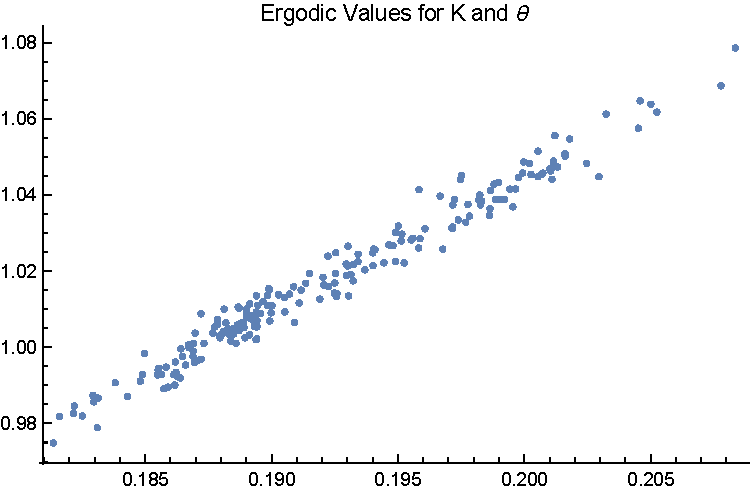
\includegraphics[width=2.3in]{ergodicKTheta.pdf}
  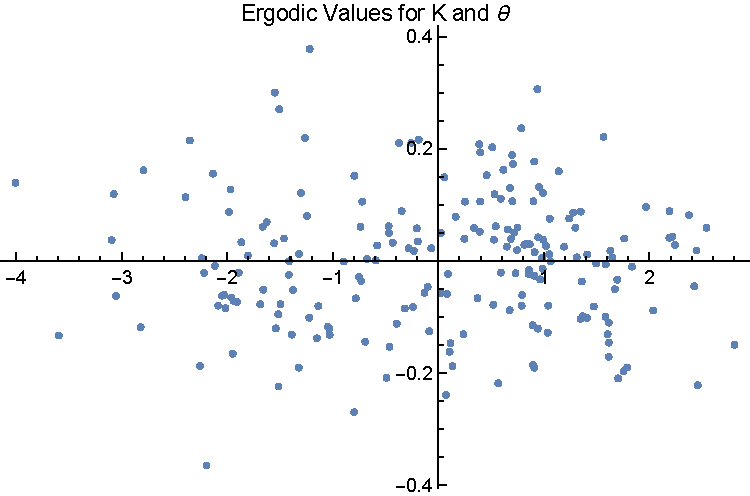
\includegraphics[width=2.3in]{ergodicZs.pdf}
  \caption{The Ergodic Values for $k_t, \theta_t$ }
  \label{fig:erg}
\end{figure}


\begin{gather}
\bar{X}= \vcenter{\hbox{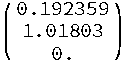
\includegraphics{ergodicMean.pdf}}}
\end{gather}
\begin{gather}
\sigma_{X}= \vcenter{\hbox{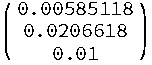
\includegraphics{ergodicSD.pdf}}}
\end{gather}


\begin{gather}
V= \vcenter{\hbox{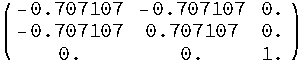
\includegraphics{ergodicV.pdf}}}
\end{gather}

\begin{gather}
\max U= \vcenter{\hbox{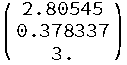
\includegraphics{ergodicMaxZ.pdf}}}
\end{gather}
\begin{gather}
\min U= \vcenter{\hbox{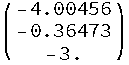
\includegraphics{ergodicMinZ.pdf}}}
\end{gather}


Table \ref{evalpA} shows the evaluation points when the Smolyak polynomial 
degrees of approximation
were (1,1,1).  Table \ref{valatA} shows the decision rule prescription for $(c_t,k_t,\theta_t)$ at each evaluation point. Table \ref{acterrA} shows the log of the absolute value of the actual error in the decision rule
at each evaluation point.  Table \ref{esterrA} shows the 
log of the absolute value of the estimated error in the decision rule
at each evaluation points.  Note that the formula provides accurate estimates
of the error component by component.



Table \ref{evalpB} shows the evaluation points when the Smolyak polynomial 
degrees of approximation
were (2,2,2).  Table \ref{valatB} shows the decision rule prescription for $(c_t,k_t,\theta_t)$ at each evaluation point. Table \ref{acterrB} shows the log of the absolute value of the actual error in the decision rule
at each evaluation point.  Table \ref{esterrB} shows the 
log of the absolute value of the estimated error in the decision rule
at each evaluation points.  Note that the formula provides accurate estimates
of the error component by component. Each of the estimated errors were computed with $K=5$.


 \begin{table}
   \centering
  
 \begin{gather*}
   \begin{bmatrix}
     k_1&\theta_1&\theShock_1\\
 &\vdots\\
     k_{30}&\theta_{30}&\theShock_{30}\\
   \end{bmatrix}\\
%  \input{xs1x1x1x5}
 \end{gather*}\\
   \caption{RBC Known Solution: Model Evaluation Points \label{evalpA} d=(1,1,1)}
 \end{table}


\begin{table}
  \centering
  
\begin{gather*}
  \begin{bmatrix}
    c_1&k_1&\theta_1\\
&\vdots\\
    c_{30}&k_{30}&\theta_{30}\\
  \end{bmatrix}\\
%  \input{theApps1x1x1x5}
\end{gather*}\\
  \caption{RBC Known Solution: Values at Evaluation Points \label{valatA} d=(1,1,1)}
\end{table}

 \begin{table}
    \centering
   \begin{gather*}
\forActErr\\
%  \input{actErrs1x1x1x5}
   \end{gather*}\\
   \caption{RBC Known Solution: Actual Errors\label{acterrA} d=(1,1,1)}
 \end{table}

 \begin{table}
   \centering
  
   \begin{gather*}
\forEstErr\\
%   \input{errs1x1x1x5}
   \end{gather*}\\
   \caption{RBC Known Solution: Error Approximations\label{esterrA} d=(1,1,1)}
 \end{table}


\begin{table}
  \centering
  
\begin{gather*}
  \begin{bmatrix}
    k_1&\theta_1&\theShock_1\\
&\vdots\\
    k_{30}&\theta_{30}&\theShock_{30}\\
  \end{bmatrix}\\
%  \input{xs2x2x2x5}
\end{gather*}\\
  \caption{RBC Known Solution: Model Evaluation Points \label{evalpB} d=(2,2,2)}
\end{table}

\begin{table}
  \centering
  
\begin{gather*}
  \begin{bmatrix}
    k_1&\theta_1&\theShock_1\\
&\vdots\\
    k_{30}&\theta_{30}&\theShock_{30}\\
  \end{bmatrix}\\
%  \input{xs2x2x2x5}
\end{gather*}\\
  \caption{RBC Known Solution: Values at Evaluation Points \label{valatB}d=(2,2,2)}
\end{table}


 \begin{table}
    \centering
   \begin{gather*}
\forActErr\\
%  \input{actErrs2x2x2x5}
   \end{gather*}\\
   \caption{RBC Known Solution: Actual Errors\label{acterrB}d=(2,2,2)}
 \end{table}

 \begin{table}
   \centering
  
   \begin{gather*}
\forEstErr\\
%   \input{errs2x2x2x5}
   \end{gather*}\\
   \caption{RBC Known Solution: Error Approximations\label{esterrB}d=(2,2,2)}
 \end{table}


Table \ref{impactK} shows the effect of increasing value of K.  Generally
increasing K increases the accuracy of the solution.  The value of K has
more effect when the Smolyak grid is more densely populated with collocation
points.



 \begin{table}
   \centering
   \begin{gather*}
          \begin{bmatrix}
       K&d=(1,1,1)&d=(2,2,2)&d=(3,3,3)
     \end{bmatrix}\\
   \end{gather*}
%\vspace{.2in}
   \begin{gather*}
%   \input{errByKTab}     
   \end{gather*}
   \caption{RBC Known Solution: Impact of Series Length on Approximation Error \label{impactK}}
 \end{table}



\clearpage
\subsection{Approximating an Unknown Solution: $\eta=3$ }
\label{sec:recov-unknown-solut}


Table \ref{evalpunkA} shows the evaluation points when the Smolyak polynomial 
degrees of approximation
were (1,1,1).  Table \ref{valatunkA} shows the decision rule prescription for $(c_t,k_t,\theta_t)$ at each evaluation point.   Table \ref{esterrunkA} shows the 
log of the absolute value of the estimated error in the decision rule
at each evaluation points.  Note that the formula provides accurate estimates
of the error component by component.



Table \ref{evalpunkB} shows the evaluation points when the Smolyak polynomial 
degrees of approximation
were (2,2,2).  Table \ref{valatunkB} shows the decision rule prescription for $(c_t,k_t,\theta_t)$ at each evaluation point.   Table \ref{esterrB} shows the 
log of the absolute value of the estimated error in the decision rule
at each evaluation points.  Note that the formula provides accurate estimates
of the error component by component.

 \begin{table}
   \centering
  
 \begin{gather*}
   \begin{bmatrix}
     k_1&\theta_1&\theShock_1\\
 &\vdots\\
     k_{30}&\theta_{30}&\theShock_{30}\\
   \end{bmatrix}\\
%  \input{xs1x1x1x5Unk}
 \end{gather*}\\
   \caption{RBC Approximated Solution: Model Evaluation Points \label{evalpunkA} d=(1,1,1)}
 \end{table}


\begin{table}
  \centering
  
\begin{gather*}
  \begin{bmatrix}
    c_1&k_1&\theta_1\\
&\vdots\\
    c_{30}&k_{30}&\theta_{30}\\
  \end{bmatrix}\\
%  \input{theApps1x1x1x5Unk}
\end{gather*}\\
  \caption{RBC Approximated Solution: Values at Evaluation Points \label{valatunkA} d=(1,1,1)}
\end{table}

 \begin{table}
   \centering
  
   \begin{gather*}
\forEstErr
\\
%   \input{errs1x1x1x5Unk}
   \end{gather*}\\
   \caption{RBC Approximated Solution: Error Approximations\label{esterrunkA} d=(1,1,1)}
 \end{table}


\begin{table}
  \centering
  
\begin{gather*}
  \begin{bmatrix}
    k_1&\theta_1&\theShock_1\\
&\vdots\\
    k_{30}&\theta_{30}&\theShock_{30}\\
  \end{bmatrix}\\
%  \input{xs2x2x2x5Unk}
\end{gather*}\\
  \caption{RBC Approximated Solution: Model Evaluation Points \label{evalpunkB} d=(2,2,2)}
\end{table}

\begin{table}
  \centering
  
\begin{gather*}
  \begin{bmatrix}
    k_1&\theta_1&\theShock_1\\
&\vdots\\
    k_{30}&\theta_{30}&\theShock_{30}\\
  \end{bmatrix}\\
%  \input{theApps2x2x2x5Unk}
\end{gather*}\\
  \caption{RBC Approximated Solution: Values at Evaluation Points \label{valatunkB}d=(2,2,2)}
\end{table}



 \begin{table}
   \centering
  
   \begin{gather*}
\forEstErr\\
%   \input{errs2x2x2x5Unk}
   \end{gather*}\\
   \caption{RBC Approximated Solution: Error Approximations\label{esterrunkB}d=(2,2,2)}
 \end{table}


\clearpage
\section{A Model with Occasionally Binding Constraints}
\label{sec:occbind}



\label{sec:obc-solut}

Stochastic dynamic non linear economic
models often embody  occasionally binding constraints (OBC).
Since  \citep{Christiano2000} a host of
authors have described a variety of approaches.\footnote{The algorithms described in  \citep{holden15:_exist_dsge} and  \citep{guerrieri15:_occbin} also exploit the use of ``anticipated shocks'', but do not use the comprehensive formula employed here. }
 \citep{holden15:_exist_dsge,guerrieri15:_occbin,benigno09,hintermaier10,brumm10,nakov08,haefke98,nakata12,gordon11,billi11,Hintermaier2010,Guerrieri2015}


%\subsection{First Order Conditions Lagrangian Derivations}
\label{sec:folag}

Consider adding  a  constraint to the simple RBC model:

\begin{gather*}
  I_t \ge \upsilon I_{ss}
\end{gather*}


 \begin{gather*}
   \max\left \{  u(c_t) + E_t \sum_{t=0}^\infty  \delta^{t+1}u(c_{t+1})\right \}\\
   c_t + k_t=(1-d)k_{t-1} + \theta_t f(k_{t-1})\\
    \theta_t =\theta_{t-1}^\rho e^{\theShock_t}\\
f(k_t)= k_t^\alpha\\
u(c)=\frac{c^{1-\eta}-1}{1-\eta}\\
 \mathbb{L}= \left \{ 
 u(c_t)+E_t\sum_{t=0}^\infty \delta^{t}u(c_{t+1}) 
 \right \}+ \\
\sum_{t=0}^\infty 
\left \{ \delta^t \lambda_t  (c_t + k_t-((1-d)k_{t-1} + \theta_t f(k_{t-1}))) + \right . \\ 
\left . \delta^t \mu_t( (k_t - (1-d)k_{t-1} ) - \upsilon I_{ss})  \right \} \intertext{ so that we can impose}
 I_t =(k_t - (1-d)k_{t-1} ) \ge  \upsilon I_{ss}\intertext{ The first order conditions become}
\frac{1}{c_t^\eta} + \lambda_t\\
\lambda_t - \delta \lambda_{t+1}\theta_{t+1} \alpha k_t^{(\alpha-1)}- \delta(1-d) \lambda_{t+1} + \mu_t - \delta (1-d)\mu_{t+1}
% \intertext{To computed the bordered Hessian we need}
% \nabla G_1=\nabla
% \begin{bmatrix}
% (c_t + k_t-((1-d)k_{t-1} + \theta_t f(k_{t-1})))\\
% -(c_t + k_t-((1-d)k_{t-1} + \theta_t f(k_{t-1})))\\
% (c_{t+1} + k_{t+1}-((1-d)k_{t} + \theta_{t+1} f(k_{t})))\\
% -(c_{t+1} + k_{t+1}-((1-d)k_{t} + \theta_{t+1} f(k_{t})))
% \end{bmatrix}=\\
% \begin{bmatrix}
%   1&1\\
%   -1&-1\\
% 0&(1-d)+\theta_{t+1}\alpha k_t^{(\alpha-1)}\\
% 0&-((1-d)+\theta_{t+1}\alpha k_t^{(\alpha-1)})
% \end{bmatrix}\\
% \nabla G_2=\nabla
% \begin{bmatrix}
% (c_t + k_t-((1-d)k_{t-1} + \theta_t f(k_{t-1})))\\
% -(c_t + k_t-((1-d)k_{t-1} + \theta_t f(k_{t-1})))\\
% (c_{t+1} + k_{t+1}-((1-d)k_{t} + \theta_{t+1} f(k_{t})))\\
% -(c_{t+1} + k_{t+1}-((1-d)k_{t} + \theta_{t+1} f(k_{t})))\\
% ( (k_t - (1-d)k_{t-1} ) - \upsilon I_{ss})\\
% ( (k_{t+1} - (1-d)k_{t} ) - \upsilon I_{ss})
% \end{bmatrix}
% \intertext{The second order conditions are}
% \begin{bmatrix}
% -\eta c^{-(\eta+1)}&0\\
% 0& \alpha(\alpha-1) k_t^{(\alpha-2)}
% \end{bmatrix}
\end{gather*}


For example, the Euler equations for the  neoclassical growth  model 
%\label{sec:simple-rbc-model-ext}
can be written as
 


\begin{tcolorbox}[ams gather]
if(\mu>0 \land (k_t - (1-d)k_{t-1}-\upsilon I_{ss})=0)\\
  \lambda_t -\frac{1}{c_t}\\
c_t+I_t-\theta_tk_{t-1}^\alpha\\
N_t-\lambda_t \theta_t\\
\theta_t-e^{(\rho\ln(\theta_{t-1})+\theShock)}\\
\lambda_t + \mu_t - (\alpha k_t^{(\alpha-1)}\delta N_{t+1}+\lambda_{t+1} \delta (1-d)+\mu_{t+1}+\delta (1-d)\mu_{t+1}\\
I_t-(K_t-(1-d)k_{t-1})\\
\mu_t(k_t - (1-d) k_{t-1}-\upsilon I_{ss})\\
\end{tcolorbox}
\begin{tcolorbox}[ams gather]
if(\mu=0 \land (k_t - (1-d)k_{t-1}-\upsilon I_{ss})\ge 0)\\
  \lambda_t -\frac{1}{c_t}\\
c_t+I_t-\theta_tk_{t-1}^\alpha\\
N_t-\lambda_t \theta_t\\
\theta_t-e^{(\rho\ln(\theta_{t-1})+\theShock)}\\
\lambda_t + {\mu_t} - (\alpha k_t^{(\alpha-1)}\delta N_{t+1}+\lambda_{t+1} \delta (1-d)+{\mu_{t+1}}+\delta (1-d)\mu_{t+1}\\
I_t-(K_t-(1-d)k_{t-1})\\
\mu_t(k_t - (1-d) k_{t-1}-\upsilon I_{ss})
\end{tcolorbox}



Table \ref{evalpobcA} shows the evaluation points when the Smolyak polynomial 
degrees of approximation
were (1,1,1).  Table \ref{valatobcA} shows the decision rule prescription for $(c_t,k_t,\theta_t)$ at each evaluation point.   Table \ref{esterrobcA} shows the 
log of the absolute value of the estimated error in the decision rule
at each evaluation points.  Note that the formula provides accurate estimates
of the error component by component.



Table \ref{evalpobcB} shows the evaluation points when the Smolyak polynomial 
degrees of approximation
were (2,2,2).  Table \ref{valatobcB} shows the decision rule prescription for $(c_t,k_t,\theta_t)$ at each evaluation point.   Table \ref{esterrobcB} shows the 
log of the absolute value of the estimated error in the decision rule
at each evaluation points.  Note that the formula provides accurate estimates
of the error component by component.




 \begin{table}
   \centering
  
 \begin{gather*}
   \begin{bmatrix}
     k_1&\theta_1&\theShock_1\\
 &\vdots\\
     k_{30}&\theta_{30}&\theShock_{30}\\
   \end{bmatrix}\\
%  \input{xs1x1x1x5CS}
 \end{gather*}

   \caption{Occasionally Binding Constraints Model Evaluation Points \label{evalpobcA} d=(1,1,1)}
 \end{table}


\begin{table}
  \centering
  
\begin{gather*}
  \begin{bmatrix}
    c_1&I_1&k_1\\
&\vdots\\
    c_{30}&I_{30}&k_{30}\\
  \end{bmatrix}\\
% \input{theApps1x1x1x5CS}
\end{gather*}

  \caption{Occasionally Binding Constraints Values at Evaluation Points for Occasionally Binding Constraints \label{valatobcA}  d=(1,1,1)}
\end{table}

 \begin{table}
   \centering
  
   \begin{gather*}
\forEstErr\\
%   \input{errs1x1x1x5CS}
   \end{gather*}
   \caption{Occasionally Binding Constraints Error Approximations\label{esterrobcA}  d=(1,1,1)}
 \end{table}





 \begin{table}
   \centering
  
 \begin{gather*}
   \begin{bmatrix}
     k_1&\theta_1&\theShock_1\\
 &\vdots\\
     k_{30}&\theta_{30}&\theShock_{30}\\
   \end{bmatrix}\\
%  \input{xs2x2x2x5CS}
 \end{gather*}

   \caption{Occasionally Binding Constraints Model Evaluation Points \label{evalpobcB} d=(2,2,2)}
 \end{table}


\begin{table}
  \centering
  
\begin{gather*}
  \begin{bmatrix}
    k_1&\theta_1&\theShock_1\\
&\vdots\\
    k_{30}&\theta_{30}&\theShock_{30}\\
  \end{bmatrix}\\
% \input{theApps2x2x2x5CS}
\end{gather*}

  \caption{Occasionally Binding Constraints Values at Evaluation Points for Occasionally Binding Constraints \label{valatobcB}  d=(2,2,2)}
\end{table}


 \begin{table}
   \centering

   \begin{gather*}
\forEstErr\\
%   \input{errs2x2x2x5CS}
   \end{gather*}
   \caption{Occasionally Binding Constraints Error Approximations\label{esterrobcB}  d=(2,2,2)}
 \end{table}

Why not here?



\clearpage
\section{Conclusions}
This paper introduces a new series representation for bounded time series and
shows how to develop  series for representing bounded time invariant maps.
The series representation plays a strategic role in developing a formula 
for approximating the errors in dynamic model solution decision rules. 
 The paper
also shows how to  augment the usual ``Euler Equation'' model solution
methods with constraints reflecting how the updated
conditional expectation paths relate to the time t solution values thereby
enhancing solution algorithm reliability and accuracy.
The prototype was written in Mathematica and is available on gitHub
at \href{https://github.com/es335mathwiz/AMASeriesRepresentation}{https://github.com/es335mathwiz/AMASeriesRepresentation}.

{\color{blue}
It would be interesting to apply the techniques in a recent paper, \href{https://github.com/dreossi/sapo}{DreossiDP16, describing a method for characterizing thefamilies of trajectories ``reachable'' for a given set of initial conditions}.
It would be useful to apply the error fomulas to decision rules generated
using local perturbation techniques and to explore ways to use the series
representation to improve upon the accuracy of these methods.

Timing comparisons and impact of parallelism.
}
\newpage

% There are many directions to pursue in future work.
% The technique should be useful for value function iteration.
% I have begun work  developing a Julia version.
% In writing  Mathematica code I applied a functional programming style
% while blending numerica and symbolic calculations. Along with
% Mathematica, Julia is also a homoiconic language where functions are first order objects. But, I suspect that the 
% symbolic numeric balance may be different as I implement the code in Julia.
% Indeed, perhaps the Julia code will be completely numeric.
% In that implementation, I 
% will investigate computational efficiency issues and further
% exploit the high degree of parallelism available in the algorithm.

%Using tail contribution can reduce magnitude of $z_0$

% \begin{description}
% \item[Series Unique] Provides mechanism for bounding solutions
% \item[augmenting traditional] provides basis for augmenting traditional techniques
% \item[important constraint] identifies important and useful constraint on solutions
% \item[\href{https://github.com/es335mathwiz/AMASeriesRepresentation.git}{github access}] 
% \end{description}
\label{sec:conc}




\bibliographystyle{plainnat}
\bibliography{anderson,files}
%\bibliography{files}
\newpage

\clearpage
\appendix


\section{Error Approximation Formula Proof}
\label{sec:error-bound-formula}


We consider time invariant maps such as often arise from solving an
 optimization problem codified in a systems of equations.  
In what follows, we construct an error approximation for proposed model solutions.
Consider a bounded region, $\bndRgn$, where all iterated conditional expectations paths remain bounded.
 Given an exact solution $x^\star_t=g^\star(x_{t-1},\theShock_t)$ define the conditional expectations function,
  \begin{gather}
G^\star(x)\equiv\expct{g^\star(x,\theShock)} \intertext{then with}
E_tx^\star_{t+1}=G^\star(g^\star(x_{t-1},\theShock_t)) \intertext{we have}
    \eqnFunc(x^\star_{t-1},x^\star_t,E_tx^\star_{t+1},\theShock_t)=0  \,\, \forall  (x_{t-1},\theShock_t)\\ \intertext{In words, the exact solution  exactly satisfies the model equations.  Using $G^\star$ and $\linMod$, construct the family of trajectories and corresponding $z^\star_t(x_{t-1},\theShock)$ }
   x^\star_t(x_{t-1},\theShock_t) \in{R^L}\,\,\twoNorm{x^\star_t(x_{t-1},\theShock_t)}  \le \bar{\mathcal{X}}\,\,\forall t\ > 0
  \end{gather}
   \begin{align}
   z^\star_{t}(x_{t-1},\theShock_t) \equiv& H_{-1}  x^\star_{t-1}(x_{t-1},\theShock_t) + \nonumber\\
 & H_0  x^\star_{t}(x_{t-1},\theShock_t) +   \\
 & H_1  x^\star_{t+1}(x_{t-1},\theShock_t). \nonumber
   \end{align}




   Consequently, the exact solution has a representation given by
	 \begin{gather}
	 x^\star_{t}(x_{t-1},\theShock) =B x_{t-1}+ \phiMat \psiEpsMat\theShock + (I - F)^{-1} \phiMat \psiCMat +\\ \sum_{\sumIdx=0}^\infty F^s \phiMat z^\star_{t+\sumIdx}(x_{t-1},\theShock) \intertext{and}
	 \expct{x^\star_{t+1}(x_{t-1},\theShock)} =B x^\star_{t+k} + \sum_{\sumIdx =0}^\infty F^\sumIdx \phiMat \expct{z^\star_{t+1+\sumIdx}(x_{t-1},\theShock)} + (I - F)^{-1} \phiMat \psiCMat 
 \intertext{with}
 \eqnFunc(x_{t-1},x^\star_t,E_tx^\star_{t+1},\theShock_t)=0  \,\, \forall  (x_{t-1},\theShock_t)\\ 
	 \end{gather}

Now consider a proposed solution for the model,
 $x^p_t=g^p(x_{t-1},\theShock_t)$ define
$G^p(x)\equiv\expct{g^p(x,\theShock)}$  so that 
  \begin{gather*}
E_tx_{t+1}=G^p(g^p(x_{t-1},\theShock_t))\\
\mathbf{e}_t^p(x_{t-1},\theShock)\equiv
\eqnFunc(x_{t-1},x^p_t,E_tx^p_{t+1},\theShock_t)
\end{gather*}
By construction,  the conditional expectations paths will all be bounded
in the region $\bndRgn^p$. Using $G^p$ and $\linMod$ construct the family of trajectories and corresponding $z^p_t(x_{t-1},\theShock)$\footnote{The algorithm presented below for finding solutions provides a mechanism for generating such proposed solutions.} 
\begin{gather*}
   x^p_t(x_{t-1},\theShock_t) \in{R^L}\,\,\twoNorm{x^p_t(x_{t-1},\theShock_t)}  \le \bar{\mathcal{X}}\,\,\forall t\ > 0
  \end{gather*}
   \begin{align}
   z^p_{t}(x_{t-1},\theShock_t) \equiv& H_{-1}  x^p_{t-1}(x_{t-1},\theShock_t) + \nonumber\\
 & H_0  x^p_{t}(x_{t-1},\theShock_t) +   \\
 & H_1  x^p_{t+1}(x_{t-1},\theShock_t). \nonumber
   \end{align}








 The proposed solution has a representation given by 
  \begin{gather}
    \label{eq:4}
	 x^p_{t}(x_{t-1},\theShock) =B x_{t-1}+ \phiMat \psiEpsMat\theShock + (I - F)^{-1} \phiMat \psiCMat +\\ \sum_{\sumIdx=0}^\infty F^s \phiMat z^p_{t+\sumIdx}(x_{t-1},\theShock) 
 \intertext{and}
 	 \expct{x^p_{t+1}(x_{t-1},\theShock)} =B x^p_{t+k} + \sum_{\sumIdx =0}^\infty F^\sumIdx \phiMat z^p_{t+1+\sumIdx}(x_{t-1},\theShock) + (I - F)^{-1} \phiMat \psiCMat \intertext{with}
\mathbf{e}_t^p(x_{t-1},\theShock)\equiv
\eqnFunc(x_{t-1},x^p_t,E_tx^p_{t+1},\theShock_t)
  \end{gather}




  \begin{gather}
    \label{eq:3}
	 x^\star_{t}(x_{t-1},\theShock) -	 x^p_{t}(x_{t-1},\theShock) =
         \sum_{\sumIdx=0}^\infty F^s \phiMat (z^\star_{t+\sumIdx}(x_{t-1},\theShock)-z^p_{t+\sumIdx}(x_{t-1},\theShock))     \\
\Delta z_{t+\sumIdx}^p(x_{t-1},\theShock_t)         \equiv (z^\star_{t+\sumIdx}(x_{t-1},\theShock)-z^p_{t+\sumIdx}(x_{t-1},\theShock))\\
	 x^\star_{t}(x_{t-1},\theShock) -	 x^p_{t}(x_{t-1},\theShock) =
\sum_{\sumIdx=0}^\infty F^s \phiMat \Delta z_{t+\sumIdx}^p(x_{t-1},\theShock_t)   \\ 
	\infNorm{ x^\star_{t}(x_{t-1},\theShock) -	 x^p_{t}(x_{t-1},\theShock)} \le
\sum_{\sumIdx=0}^\infty F^s \phiMat \infNorm{\Delta z_{t+\sumIdx}^p(x_{t-1},\theShock_t)}    
  \end{gather}

  By bounding the largest deviation in the paths for the $\Delta z_t^p$ we can bound the largest difference in $x_t$.\footnote{Since the future values are probability weighted averages of the $\Delta z_t^p$ values for the given initial conditions and the condition expectations paths remain in the region $\bndRgn^p$,
the largest error for $\Delta z_{t+k}^p$   are pessimistic bounds for the errors from the conditional expectations path. } The exact solution satisfies the model equations exactly.  The error associated with the proposed solution leads to a conservative bound on the largest change in $z$ needed to match the exact solution.

%error  in formula phi should multiply delta z's
{\small
  \begin{tcolorbox}[ams gather]
  \Delta z_t \le  
\max_{\{x_{-},\theShock\}} \twoNorm{ \phiMat \eqnFunc(x_{-},g^p(x_{-},\theShock),G^p(g^p(x_{-},\theShock)),\theShock) }\\
	\infNorm{ x^\star_{t}(x_{t-1},\theShock) -	 x^p_{t}(x_{t-1},\theShock)} \le
\max_{\{x_{-},\theShock\}} \twoNorm{(I-F)^{-1} \phiMat \eqnFunc(x_{-},g^p(x_{-},\theShock),G^p(g^p(x_{-},\theShock)),\theShock) }
  \end{tcolorbox}
}

\newcommand{\hApp}[1]{{H_-{#1}_{t-1} +H_0{#1}_t +H_+{#1}_{t+1}}}

 \begin{gather*}
z^\star_t=\hApp{x^\star}\\
z^p_t=\hApp{x^p}\\
0=\eqnFunc(x^\star_{t-1},x^\star_{t},x^\star_{t+1},\theShock_t)\\
\mathbf{e}_t^p(x_{t-1},\theShock)=\eqnFunc(x^p_{t-1},x^p_{t},x^p_{t+1},\theShock_t)\\
\max_{x_{t-1},\theShock_t} (\twoNorm{\phiMat \Delta z_t})^2 =\max_{x_{t-1},\theShock_t} (\phiMat(H_0(x^p_t-x^\star_t)+H_+(x^p_{t+1}-x^\star_{t+1})))^2
\intertext{with}
\eqnFunc(x^\star_{t-1},x^\star_{t},x^\star_{t+1},\theShock_t) =0\\
%\le \mathbf{e}_t^p(x_{t-1},\theShock)\\
\Delta \mathbf{e}_t^p(x_{t-1},\theShock)\approx \pdrv{\eqnFunc(x_{t-1},x_{t},x_{t+1},\theShock_t)}{x_t} (x^\star_t-x^p_t) +\pdrv{\eqnFunc(x_{t-1},x_{t},x_{t+1},\theShock_t)}{x_{t+1}} (x^\star_{t+1}-x^p_{t+1}) \intertext{ when $\pdrv{\eqnFunc(x_{t-1},x_{t},x_{t+1},\theShock_t)}{x_t}$ is non-singular, we can write}
 (x^\star_t-x^p_t) \approx \left ( \pdrv{\eqnFunc(x_{t-1},x_{t},x_{t+1},\theShock_t)}{x_t}\right )^{-1} \left ( \Delta \mathbf{e}_t^p(x_{t-1},\theShock) -\pdrv{\eqnFunc(x_{t-1},x_{t},x_{t+1},\theShock_t)}{x_{t+1}} (x^\star_{t+1}-x^p_{t+1}) \right )
\intertext{ collecting results}
 (\twoNorm{\phiMat \Delta z_t})^2 =\\ 
 (\phiMat(
H_0\left ( \pdrv{\eqnFunc(x_{t-1},x_{t},x_{t+1},\theShock_t)}{x_t}\right )^{-1} \\
\left ( \Delta \mathbf{e}_t^p(x_{t-1},\theShock) -
\pdrv{\eqnFunc(x_{t-1},x_{t},x_{t+1},\theShock_t)}{x_{t+1}} (x^\star_{t+1}-x^p_{t+1}) \right )+
H_+(x^p_{t+1}-x^\star_{t+1})))^2=
\\
 (\phiMat(
H_0\left ( \pdrv{\eqnFunc(x_{t-1},x_{t},x_{t+1},\theShock_t)}{x_t}\right )^{-1} 
( \Delta \mathbf{e}_t^p(x_{t-1},\theShock) )
-\\
\left ( H_0\left ( \pdrv{\eqnFunc(x_{t-1},x_{t},x_{t+1},\theShock_t)}{x_t}\right )^{-1} 
\pdrv{\eqnFunc(x_{t-1},x_{t},x_{t+1},\theShock_t)}{x_{t+1}} (x^\star_{t+1}-x^p_{t+1}) \right )+
H_+(x^p_{t+1}-x^\star_{t+1})))^2=\\
 (\phiMat(
H_0\left ( \pdrv{\eqnFunc(x_{t-1},x_{t},x_{t+1},\theShock_t)}{x_t}\right )^{-1} 
( \Delta \mathbf{e}_t^p(x_{t-1},\theShock) )
-\\
\left ( H_0\left ( \pdrv{\eqnFunc(x_{t-1},x_{t},x_{t+1},\theShock_t)}{x_t}\right )^{-1} 
\pdrv{\eqnFunc(x_{t-1},x_{t},x_{t+1},\theShock_t)}{x_{t+1}}  -H_+\right ) (x^\star_{t+1}-x^p_{t+1})
))^2=\intertext{approximating the derivatives using the $H$ matrices}
\pdrv{\eqnFunc(x_{t-1},x_{t},x_{t+1},\theShock_t)}{x_{t}} \approx H_0\\
\pdrv{\eqnFunc(x_{t-1},x_{t},x_{t+1},\theShock_t)}{x_{t+1}} \approx H_+\\
\intertext{produces}
\max_{x_{t-1},\theShock_t} (\phiMat \Delta \mathbf{e}_t^p(x_{t-1},\theShock))^2
  \end{gather*}




% Use Cluster MSNTO to find constrained max.  Should parallelize well.


% \begin{verbatim}
% Nelder–Mead

% The Nelder–Mead method is a direct search method. For a function of variables, the algorithm maintains a set of points forming the vertices of a polytope in -dimensional space. This method is often termed the "simplex" method, which should not be confused with the well-known simplex method for linear programming.

% At each iteration, points form a polytope. The points are ordered so that A new point is then generated to replace the worst point

% Let be the centroid of the polytope consisting of the best points, . A trial point is generated by reflecting the worst point through the centroid, , where is a parameter.

% If the new point is neither a new worst point nor a new best point, , replaces .

% If the new point is better than the best point, , the reflection is very successful and can be carried out further to , where is a parameter to expand the polytope. If the expansion is successful, , replaces ; otherwise the expansion failed, and replaces .

% If the new point is worse than the second worst point, , the polytope is assumed to be too large and needs to be contracted. A new trial point is defined as

% where is a parameter. If , the contraction is successful, and replaces . Otherwise a further contraction is carried out.

% The process is assumed to have converged if the difference between the best function values in the new and old polytope, as well as the distance between the new best point and the old best point, are less than the tolerances provided by AccuracyGoal and PrecisionGoal.

% Strictly speaking, Nelder–Mead is not a true global optimization algorithm; however, in practice it tends to work reasonably well for problems that do not have many local minima.
% \end{verbatim}


% \begin{itemize}
% \item rank condition on $\psiCMat$
% \item appendix derivations with all lagrangians
% \end{itemize}

% \section{Function Approximation Representation}
% \label{sec:funcApproxRep}

% \subsection{General Issues}
% \label{sec:generalissues}





\section{A Regime Switching Example}
\label{sec:extension}
\label{sec:ressw}



%\subsection{Regime Switching}





\label{sec:regime-switch-model}

To apply the series formula, one must construct conditional expectations paths from each initial $x(x_{t-1},\theShock_t)$.  Consider the case when the transition 
probabilities $p_{ij}$ are constant and do not depend on 
$x_{t-1},\theShock_t,x_t$.

\begin{gather*}
E_t[x_{t+1}]=  \sum_{j=1}^{N} p_{ij} E_t(x_{t+1}(x_t)|s_{t+1}=j)  \\
E_t[x_{t+2}]=  \sum_{j=1}^{N} p_{ij} E_t(x_{t+2}(x_{t+1})|s_{t+2}=j)  \\
\end{gather*}

If we know the current state we can use the known conditional expectation function for the state:
\begin{gather*}
    \begin{bmatrix}
E_t(x_{t+1}(x_{t})|s_{t}=1)  \\    \vdots \\
E_t(x_{t+1}(x_{t})|s_{t}=N)  
  \end{bmatrix}
\end{gather*}

For the next state we can compute expectations if the errors are independent
\begin{gather*}
  \begin{bmatrix}
E_t(x_{t+2}(x_t)|s_{t}=1)  \\    \vdots \\
E_t(x_{t+2}(x_t)|s_{t}=N)  
  \end{bmatrix}=
(P \otimes  I)
  \begin{bmatrix}
E_t(x_{t+2}(x_{t+1})|s_{t+1}=1)  \\    \vdots \\
E_t(x_{t+2}(x_{t+1})|s_{t+1}=N)  
  \end{bmatrix}
\end{gather*}

Consider two states $s_t \in {0,1}$ where the depreciation rates are different:  $d_0>d_1$

\begin{gather}
    Prob(s_t=j|s_{t-1}=i)=p_{ij}
\end{gather}


\begin{tcolorbox}[ams gather]
if(s_t=0\land \mu>0 \land (k_t - (1-d_0)k_{t-1}-\upsilon I_{ss})=0)\\
  \lambda_t -\frac{1}{c_t}\\
c_t+k_t-\theta_tk_{t-1}^\alpha\\
N_t-\lambda_t \theta_t\\
\theta_t-e^{(\rho\ln(\theta_{t-1})+\theShock)}\\
\lambda_t + {\mu_t} - (\alpha k_t^{(\alpha-1)}\delta N_{t+1}+\lambda_{t+1} \delta (1-d_0)+{\mu_{t+1}}+\delta (1-d_0)\\
I_t-(K_t-(1-d_0)k_{t-1})\\
\mu_t(k_t - (1-d_0) k_{t-1}-\upsilon I_{ss})\\
\end{tcolorbox}
\begin{tcolorbox}[ams gather]
if(s_t=0\land\mu=0 \land (k_t - (1-d_0)k_{t-1}-\upsilon I_{ss})\ge 0)\\
  \lambda_t -\frac{1}{c_t}\\
c_t+k_t-\theta_tk_{t-1}^\alpha\\
N_t-\lambda_t \theta_t\\
\theta_t-e^{(\rho\ln(\theta_{t-1})+\theShock)}\\
\lambda_t + {\mu_t} - (\alpha k_t^{(\alpha-1)}\delta N_{t+1}+\lambda_{t+1} \delta (1-d_0)+{\mu_{t+1}}+\delta (1-d_0)\\
I_t-(K_t-(1-d_0)k_{t-1})\\
\mu_t(k_t - (1-d_0) k_{t-1}-\upsilon I_{ss})
\end{tcolorbox}
\begin{tcolorbox}[ams gather]
if(s_t=1\land \mu>0 \land (k_t - (1-d_1)k_{t-1}-\upsilon I_{ss})=0)\\
  \lambda_t -\frac{1}{c_t}\\
c_t+k_t-\theta_tk_{t-1}^\alpha\\
N_t-\lambda_t \theta_t\\
\theta_t-e^{(\rho\ln(\theta_{t-1})+\theShock)}\\
\lambda_t + {\mu_t} - (\alpha k_t^{(\alpha-1)}\delta N_{t+1}+\lambda_{t+1} \delta (1-d_1)+{\mu_{t+1}}+\delta (1-d_1)\\
I_t-(K_t-(1-d_1)k_{t-1})\\
\mu_t(k_t - (1-d_1) k_{t-1}-\upsilon I_{ss})\\
\end{tcolorbox}
\begin{tcolorbox}[ams gather]
if(s_t=1\land\mu=0 \land (k_t - (1-d_1)k_{t-1}-\upsilon I_{ss})\ge 0)\\
  \lambda_t -\frac{1}{c_t}\\
c_t+k_t-\theta_tk_{t-1}^\alpha\\
N_t-\lambda_t \theta_t\\
\theta_t-e^{(\rho\ln(\theta_{t-1})+\theShock)}\\
\lambda_t + {\mu_t} - (\alpha k_t^{(\alpha-1)}\delta N_{t+1}+\lambda_{t+1} \delta (1-d_1)+{\mu_{t+1}}+\delta (1-d_1)\\
I_t-(K_t-(1-d_1)k_{t-1})\\
\mu_t(k_t - (1-d_1) k_{t-1}-\upsilon I_{ss})
\end{tcolorbox}



% \subsection{Smolyak Interpolation}
% \label{sec:smolyakinterp}

% \paragraph{An-isotropic}
% It is possible to precompute each of the integrals. Since the solution will be linear combination of the polynomials, precomputing the polynomials means the weighted sum of the precomputed integrals will provide the integrals.
% \paragraph{Precomputing Integrals}
% \begin{algorithm}
%   \SetKwInOut{Input}{input}
%  \SetKwInOut{Output}{output}
% \Input{$\aSmolPoly$, $\smolRngs$, $\distribSpec$} 
% \Output{$\int \aSmolPoly \Pi (f_i(\theShock_i)) d\theShock_1 \ldots d\theShock_k$}
% \end{algorithm}







% \section{Multi-cluster Sequential Number Theoretic Optimization (MSNTO)}
% \label{sec:MSNTO}

% This section describes a method for finding maxima in a closed bounded domain.
% Let $D=[a,b]$ in $R^s$ where $a_i \le x_i \le b_i$. We want to find  $M=f(x^\ast)= \max_{x \in D}f(x)$.
% Th number theoretic (Quasi-Monte Carlo) approached is designed for finding optima with many local optima.  It is based on the used of space filling points. \citep{Xu2005}
% The number theoretic method of optimization includes two basic steps.
% \begin{enumerate}
% \item Choose a set $p=x_i, i=1,\dots,n$ of potential optima that are uniformly scattered.
% \item Find $M_n\text{ and } x^\ast \in p =\max_{1\le i \le n}f(x_i)$
% \end{enumerate}

% Even when choosing $p$ wisely convergence slow until  \citep{Niederreiter1983}.  They speed up the convergence by contracting the domain.
% Their algorithm discards all but the best in the domain. Must have very many points to guarantee choosing a point close to the optimum.


% MSNTO selects a finite number of sample points uniformly scattered on D.  Next it discard inferior points retaining small sample of potential maxima.  These form the clusters for the next step.  The algorithm performs a domain contraction on each of the clusters.








\newpage
% \section{The doIt Graphs}
% \label{sec:doit-graphs}

% \begin{itemize}
% \item iterations needed for convergence differ between series and traditional
% \item approx series (1,1,1),1,1  bound violated only case so far
% \item after K >2 better than traditional
% \item should do unit free
% \item perturbation solution
% \item error bounds may decrease and then start to increase with adding K or nuimber of iters  theRes has info to check iters
% \item nminimize to msnto
% \item bounds without approximation 
% \item include epsilon value in graph
% \end{itemize}

% K has no effect on traditional

% Looks like largest errors for nonzero epsilon but graph seems to indicate error at collocation point.

% Why doItApproxSeries[1*{1,1,1},1,1] not good error bound.

% Compute exact error bound.



% \newpage

% \begin{verbatim}
% doItApproxTrad[1*{1,1,1},1,0]
% \end{verbatim}

% forBetterRBC--1,1,1-Iters1theK0host-node003dnumKern16Trad.pdf

% forBetterRBC--1,1,1-Iters1theK0host-node003dnumKern16TradApprox.pdf




%   \includegraphics{resDir/forBetterRBC--1,1,1-Iters1theK0host-node014bnumKern16Trad.pdf}


%   \includegraphics{resDir/forBetterRBC--1,1,1-Iters1theK0host-node014bnumKern16TradApprox.pdf}


% \newpage
% \begin{verbatim}
% doItApproxTrad[1*{1,1,1},10,0]
% \end{verbatim}

% forBetterRBC--1,1,1-Iters10theK0host-node003dnumKern16Trad.pdf

% forBetterRBC--1,1,1-Iters10theK0host-node003dnumKern16TradApprox.pdf




%   \includegraphics{resDir/forBetterRBC--1,1,1-Iters10theK0host-node014bnumKern16Trad.pdf}

%   \includegraphics{resDir/forBetterRBC--1,1,1-Iters10theK0host-node014bnumKern16TradApprox.pdf}



% \newpage
% \begin{verbatim}
% doItApproxSeries[1*{1,1,1},1,1]
% \end{verbatim}

% forBetterRBC--1,1,1-Iters1theK1host-node014bnumKern16.pdf



% forBetterRBC--1,1,1-Iters1theK1host-node014bnumKern16Approx.pdf


%   \includegraphics{resDir/forBetterRBC--1,1,1-Iters1theK1host-node014bnumKern16Series.pdf}

%   \includegraphics{resDir/forBetterRBC--1,1,1-Iters1theK1host-node014bnumKern16SeriesApprox.pdf}





% \newpage

% \begin{verbatim}
% doItApproxSeries[1*{1,1,1},10,1]
% \end{verbatim}

% forBetterRBC--1,1,1-Iters10theK1host-node014bnumKern16.pdf



% forBetterRBC--1,1,1-Iters10theK1host-node014bnumKern16Approx.pdf


%   \includegraphics{resDir/forBetterRBC--1,1,1-Iters10theK1host-node014bnumKern16Series.pdf}

%   \includegraphics{resDir/forBetterRBC--1,1,1-Iters10theK1host-node014bnumKern16SeriesApprox.pdf}


% \newpage

% \begin{verbatim}
% doItApproxSeries[1*{1,1,1},10,2]
% \end{verbatim}

% forBetterRBC--1,1,1-Iters10theK2host-node014bnumKern16.pdf



% forBetterRBC--1,1,1-Iters10theK2host-node014bnumKern16Approx.pdf


%   \includegraphics{resDir/forBetterRBC--1,1,1-Iters10theK2host-node014bnumKern16Series.pdf}

%   \includegraphics{resDir/forBetterRBC--1,1,1-Iters10theK2host-node014bnumKern16SeriesApprox.pdf}




% \newpage

% \begin{verbatim}
% doItApproxSeries[1*{1,1,1},10,3]
% \end{verbatim}

% forBetterRBC--1,1,1-Iters10theK3host-node014bnumKern16.pdf


% forBetterRBC--1,1,1-Iters10theK3host-node014bnumKern16Approx.pdf


%   \includegraphics{resDir/forBetterRBC--1,1,1-Iters10theK3host-node014bnumKern16Series.pdf}

%   \includegraphics{resDir/forBetterRBC--1,1,1-Iters10theK3host-node014bnumKern16SeriesApprox.pdf}




% \newpage

% \begin{verbatim}
% doItApproxSeries[1*{1,1,1},10,4]
% \end{verbatim}

% forBetterRBC--1,1,1-Iters10theK4host-node014bnumKern16.pdf


% forBetterRBC--1,1,1-Iters10theK4host-node014bnumKern16Approx.pdf


%   \includegraphics{resDir/forBetterRBC--1,1,1-Iters10theK4host-node014bnumKern16Series.pdf}


%   \includegraphics{resDir/forBetterRBC--1,1,1-Iters10theK4host-node014bnumKern16SeriesApprox.pdf}





% \newpage

% \begin{verbatim}
% doItApproxSeries[1*{1,1,1},10,5]
% \end{verbatim}

% forBetterRBC--1,1,1-Iters10theK5host-node014bnumKern16.pdf



% forBetterRBC--1,1,1-Iters10theK5host-node014bnumKern16Approx.pdf


%   \includegraphics{resDir/forBetterRBC--1,1,1-Iters10theK5host-node014bnumKern16Series.pdf}

%   \includegraphics{resDir/forBetterRBC--1,1,1-Iters10theK5host-node014bnumKern16SeriesApprox.pdf}




% \newpage

% \begin{verbatim}
% doItApproxSeries[1*{1,1,1},20,5]
% \end{verbatim}

% forBetterRBC--1,1,1-Iters70theK5host-node014bnumKern16.pdf



% forBetterRBC--1,1,1-Iters70theK5host-node014bnumKern16Approx.pdf


%   \includegraphics{resDir/forBetterRBC--1,1,1-Iters70theK5host-node014bnumKern16Series.pdf}

%   \includegraphics{resDir/forBetterRBC--1,1,1-Iters70theK5host-node014bnumKern16SeriesApprox.pdf}





% \newpage


% \begin{verbatim}
% doItApproxSeries[2*{1,1,1},20,5,"Traditional"->True]
% \end{verbatim}

% forBetterRBC--4,4,4-Iters70theK5host-node014bnumKern16.pdf


% forBetterRBC--4,4,4-Iters70theK5host-node014bnumKern16Approx.pdf


%   \includegraphics{resDir/forBetterRBC--2,2,2-Iters70theK5host-node014bnumKern16Trad.pdf}

%   \includegraphics{resDir/forBetterRBC--2,2,2-Iters70theK5host-node014bnumKern16TradApprox.pdf}




% \newpage

% \begin{verbatim}
% doItApproxSeries[2*{1,1,1},20,5]
% \end{verbatim}


% forBetterRBC--2,2,2-Iters70theK5host-node014bnumKern16.pdf


% forBetterRBC--2,2,2-Iters70theK5host-node014bnumKern16Approx.pdf


%   \includegraphics{resDir/forBetterRBC--2,2,2-Iters70theK5host-node014bnumKern16Series.pdf}

%   \includegraphics{resDir/forBetterRBC--2,2,2-Iters70theK5host-node014bnumKern16SeriesApprox.pdf}





% \newpage


% \begin{verbatim}
% doItApproxSeries[3*{1,1,1},20,5,"Traditional"->True]
% \end{verbatim}

% forBetterRBC--4,4,4-Iters70theK5host-node014bnumKern16.pdf


% forBetterRBC--4,4,4-Iters70theK5host-node014bnumKern16Approx.pdf


%   \includegraphics{resDir/forBetterRBC--3,3,3-Iters70theK5host-node014bnumKern16Trad.pdf}

%   \includegraphics{resDir/forBetterRBC--3,3,3-Iters70theK5host-node014bnumKern16TradApprox.pdf}






% \newpage


% \begin{verbatim}
% doItApproxSeries[3*{1,1,1},20,5]
% \end{verbatim}

% forBetterRBC--3,3,3-Iters70theK5host-node014bnumKern16.pdf


% forBetterRBC--3,3,3-Iters70theK5host-node014bnumKern16Approx.pdf


%   \includegraphics{resDir/forBetterRBC--3,3,3-Iters70theK5host-node014bnumKern16Series.pdf}

%   \includegraphics{resDir/forBetterRBC--3,3,3-Iters70theK5host-node014bnumKern16SeriesApprox.pdf}





% % \newpage

% % \begin{verbatim}
% % doItApproxSeries[4*{1,1,1},20,5,"Traditional"->True]
% % \end{verbatim}

% % forBetterRBC--4,4,4-Iters70theK5host-node014bnumKern16.pdf


% % forBetterRBC--4,4,4-Iters70theK5host-node014bnumKern16Approx.pdf


% %   \includegraphics{resDir/forBetterRBC--4,4,4-Iters70theK5host-node014bnumKern16Trad.pdf}

% %   \includegraphics{resDir/forBetterRBC--4,4,4-Iters70theK5host-node014bnumKern16TradApprox.pdf}





% \newpage

% \begin{verbatim}
% doItApproxSeries[4*{1,1,1},20,5]
% \end{verbatim}

% forBetterRBC--4,4,4-Iters70theK5host-node014bnumKern16.pdf


% forBetterRBC--4,4,4-Iters70theK5host-node014bnumKern16Approx.pdf



%   \includegraphics{resDir/forBetterRBC--4,4,4-Iters70theK5host-node014bnumKern16Series.pdf}

%   \includegraphics{resDir/forBetterRBC--4,4,4-Iters70theK5host-node014bnumKern16SeriesApprox.pdf}

% \subsection{Ergodic Partition of Invariant Sets}
% \label{sec:ergod-part-invar}

% Following  \citep{ergodicvisual}, consider a map $T$ on a compact metric space $\mathcal{A}$ endowed with a measure $\mu$ preserved under $T$. We wish to 
% visualize invariant sets $\mathcal{B} \subseteq \mathcal{A}$.

% \begin{gather*}
%   x_{t+1} =T x_t,\in A\,\,\forall t \in Z
% \end{gather*}

% \begin{gather*}
%   x_0 \in B \implies T^t x_0 \in B \,\,\forall t \in Z
% \end{gather*}

% For ergodic invariant sets, consider $L^1$ real valued functions on A
% \begin{gather*}
%  f:A \rightarrow \mathbb{R}\in L^1(A) \iff \int_A |f(x)|dx <\infty
% \end{gather*}

% Define time average $f^\ast(x_0)$ of a function $f\in L^1(A)$ corresponding to a phase point $x_0\in A$
% \begin{gather*}
%   f^\ast(x_0)\equiv \lim_{t\rightarrow\infty} \frac{1}{t}\sum_{k=0}^{t-1}f(T^kx_0)
% \end{gather*}

% By the Ergodic Theorem, this limit exists almost everywhere ( a. e. ).
% Call map T ergodic over $B \subset A$ if for a. . point  $x_0 \in B$ time average equals the space average for every function $f \in L^1(B)$ so that there exists an
% ergodic measure.
% \begin{gather*}
% f^\ast(x_0) =\frac{1}{\mu_B(B)}\int_B f d\mu_B  
% \end{gather*}
% a.e. $B \subset A$

% This implies $f^\ast$ is a constant a. e. in $B \subset A$  almost every orbit starting in B covers B densey at the limit.  Each $f^\ast$ is an invariant function $f^\ast(x_0)= f^\ast(T^tx_0) \, \forall t$  
% The set of real numbers induces a partition of A called $\zeta_f\equiv \{B_a\}_{a\in\mathbb{R}}$ through a function $f\in L^1(A)$

% \begin{gather*}
%   B_a=(f^\ast)^{-1}(a), \,\,\forall a \in \mathbb{R}
% \end{gather*}
% Some of $B_a$ may be empty.

% \begin{gather*}
%   \mu\left (\bigcup_aB_a \right )=\mu(A),B_a\cap B_{a^\prime} = \emptyset ,\,\,\forall a \ne a^\prime
% \end{gather*}
% Denote set of points with no time average of $f$ by $\Sigma(f,T)$

% \begin{gather*}
%   A=(\cup_aB_a)\bigcup \Sigma(f,T)
% \end{gather*}
% To guarantee we don't lump what should be independent invariant sets together just because averages match, define using a collection of functions.
% Final ergodic partation $\zeta_e$ product of all $zeta_f$ belonging to $S \subset L^1(A)$  Chose S as a basis for $L^1(A)$

% \begin{gather*}
%   \zeta_e= \bigvee_{f\in S} \zeta_f
% \end{gather*}

% Ergodic partition divides phase space into non-decomposable invariant sewts.  Can visualize using approximate ergodic partitions.

% \begin{enumerate}
% \item Set up a grid of initial grid-points
% \item Pick N function $\{f_1,\ldots,f_N\}$ from $L^1(A)$ and compute partial time averages for $t_{final}$ iterations for each grid point.  These serve as approximations for $\{f_1^\ast,\ldots,f_N^\ast\}$
% \item To every initial grid point associate the corresponding time average vector
%   \begin{gather*}
%     x \rightarrow \bar{f}(x),\,\, \bar{f}(x)\equiv \{f_1^\ast(x),\ldots,f_N^\ast(x)\}\in \mathbb{R}^N
%   \end{gather*}
% \item Observe the distribution of time average vectors $\bar{f}$ and group them into clusters
% \end{enumerate}

\section{Algorithm Pseudo-code}
\label{sec:pseudocode}



\begin{description}
\item[$\linMod\equiv \linModMats$] The linear reference model
\item[$ \sVar^{p}\tArg$] The proposed decision rule  $x_t$ components
\item[$ \zVar^{p}\tArg$]The proposed decision rule  $z_t$ components
\item[$ \XVar^p\tNo$] The proposed decision rule conditional expectations  $x_t$ components
\item[$ \ZVar^p\tNo$] The proposed decision rule their conditional expectations  $z_t$ components
\item[$ \kappa$] One less than the number of terms in series representation$(\kappa>=0)$
\item[$\smolSpec$] Smolyak an-isotropic grid polynomials $(\aSmolPoly{1},\ldots,\aSmolPoly{N})$ and their conditional expectations $(\aSmolPolyCE{1},\ldots,\aSmolPolyCE{N})$
\item[$\mathbb{T}$] Model evaluation points Neidereiter sequence in the model variable ergodic region.
\item[$ \xzFunc$]  $\{\sVar\tArg,\zVar\tArg\}$ collects the decision rule components
\item[$ \XZFunc$]  $\{\sVar\tArg,\zVar\tArg\}$ collects the decision rule conditional expectations components
\item[$\bothFuncs$] $\{\xzFunc,\XZFunc\}$ collects decision rule information
\item[$\eqnFuncSys$] The equation system $\eqnFuncSig$
\end{description}
\SetKw{nestWhile}{NestWhile}
\SetKw{func}{Function}
\SetKw{map}{Map}


\begin{algorithm}
 \SetKwInOut{Input}{input}
 \SetKwInOut{Output}{output}
\Input{$(\linMod,\bothFuncs^0,\kappa,\eqnFuncSys,\smolSpec,\mathbb{T})$}
\tcc{Compute a sequence of decision rule and conditional expectation rule function terminating when the evaluation of the functions at the tests points no longer changes much. Norm of the difference controlled by default (``normConvTol''->$10^{-10} $)}
\nestWhile($\func(v,doInterp(\linMod, v, \kappa,\eqnFuncSys,\smolSpec)),\bothFuncs^0,notConvergedAt(v,\mathbb{T})$)\\
\Output{$\{\bothFuncs^0,\bothFuncs^{1},\ldots,\bothFuncs^{c}\}$}
\caption{$nestInterp$\label{nestInterp}} 
\end{algorithm}

%linMod \sVar^{p}, \zVar^{p}, \XVar^p, \ZVar^p, \kappa,


\begin{algorithm}
 \SetKwInOut{Input}{input}
 \SetKwInOut{Output}{output}
\Input{$(\linMod,\bothFuncs^i,\kappa,\eqnFuncSys,\smolSpec)$}
\tcc{Symbolically generates a collection of function triples
and an outer 
model solution selection function. Each of triples
 returns the boolean gate values and a unique value for 
$x_t$ for any given value of $(x_{t-1},\theShock_t)$ 
one of the  model equations  
and subsequently uses these 
functions to construct interpolating functions approximating the 
decision rules.}
$theFindRootFuncs=genFindRootFuncs(\linMod,\bothFuncs,\kappa,\eqnFuncSys)$\\
$\bothFuncs^{i+1}=makeInterpFuncs(theFindRootFuncs,\smolSpec)$\\
\Output{$\bothFuncs^{i+1}$}
\caption{$doInterp$\label{doInterp}} 
\end{algorithm}




\begin{algorithm}
 \SetKwInOut{Input}{input}
 \SetKwInOut{Output}{output}
\Input{$(\linMod,\bothFuncs,\kappa,\eqnFuncSys,\smolSpec)$}
\tcc{Applies genFindRootWorker to each model component.
Symbolically generates a collection of function triples
and an outer 
model solution selection function. Each of the triples
 returns the Boolean gate values and a unique value for 
$x_t$ for any given value of $(x_{t-1},\theShock_t)$ 
for one from the set of  model equations. It
 subsequently uses these 
functions to construct interpolating functions approximating the 
decision rules.
Each of the function constructions can be done in {\bf parallel}.
}
$theFuncOptionsTriples=\map(\func(v,\{v[1],genFindRootWorker(\linMod,\bothFuncs,\kappa,v[2]),v[3]),
\eqnFuncSysNoD)$\\
\Output{$\{theFuncOptionsTriples,\theD\}$}
\caption{$genFindRootFuncs$\label{genFindRootFuncs}} 
\end{algorithm}



\begin{algorithm}
 \SetKwInOut{Input}{input}
 \SetKwInOut{Output}{output}
\Input{$(\linMod,\XZFunc,\kappa,\eqnFunc)$}
\tcc{{\bf Symbolically} constructs functions that return  $x_t$ for a given
$\tArg$}
$\theZsNow=\{Z_{t+1},\ldots,Z_{t+k-1}\}=genZsForFindRoot(\linMod,x_t^p,\XZFunc)$\\
$modEqnArgsFunc=genLilXkZkFunc(\linMod,\theZsNow)$\\
$\modEqnArgsNow=\{x_{t-1},x_{t},E_t(x_{t+1}),\theShock_t\}=modEqnArgsFunc(x_{t-1},\theShock_t,z_t)$\\
$funcOfXtZt=FindRoot((x_t^p,z_t),\{\eqnFunc(\modEqnArgsNow),x_t-x_t^p\})$\\
$funcOfXtm1Eps=Function((x_{t-1},\theShock_t),funcOfXtZt)$\\
\Output{$funcOfXtm1Eps$}
\caption{$genFindRootWorker$\label{genFindRootWorker}} 
\end{algorithm}


\begin{algorithm}
 \SetKwInOut{Input}{input}
 \SetKwInOut{Output}{output}
\Input{$(x_t^p,\linMod,\XZFunc,\kappa,\eqnFunc)$}
\tcc{Symbolically compute the $\kappa-1$ future conditional Z's vectors needed for the series formula.(empty list for $\kappa=1$}
$X_{t}=x_t^p$
\For{$i=1,i<\kappa-1,i++$}{$
\{X_{t+1},Z_{t+i}\}=\XZFunc(Z_{t+i-1})
$}
$=\{(X_{t+i},Z_{t+1}),\ldots,(X_{t+\kappa-1}Z_{t+\kappa-1})\}=genZsForFindRoot(\linMod,x_t^p,\XZFunc)$\\
\Output{$\{Z_{t+1},\ldots,Z_{t+k-1}\}$}
\caption{$genZsForFindRoot$\label{genZsForFindRoot}}
\end{algorithm}



\begin{algorithm}
 \SetKwInOut{Input}{input}
 \SetKwInOut{Output}{output}
\Input{$(\linMod=\linModMats)$}
\tcc{Create functions that use the solution from the linear 
reference model for an initial proposed decision rule function and 
decision rule conditional expectation function.}
$\xzFunc(x,\theShock)=
\begin{bmatrix}
B x+(I-F)^{-1} \phiMat \psiCMat+ \psiEpsMat \theShock_t\\0_{\numZ}  
\end{bmatrix}$\\
$\XZFunc(x,\theShock)=
\begin{bmatrix}
B x+(I-F)^{-1} \phiMat \psiCMat+ \psiEpsMat \\0_{\numZ}  
\end{bmatrix}$\\
$\bothFuncs=\{\xzFunc,\XZFunc\}$\\
\Output{$\{\bothFuncs\}$}
\caption{$genBothX0Z0Funcs$\label{genBothX0Z0Funcs}} 
\end{algorithm}


\begin{algorithm}
 \SetKwInOut{Input}{input}
 \SetKwInOut{Output}{output}
\Input{$(\linMod,\{Z_{t+1},\ldots,Z_{t+k-1}\})$}
\tcc{Symbolically creates a function that uses an initial $Z_t$ path to generate a function of $(x_{t-1},\theShock_t,z_t)$ providing (potentially symbolic ) inputs $(x_{t-1},x_t,E_t(x_{t+1}),\theShock_t)$,for model system equations $\eqnFunc$} 
$fCon=fSumC(\phiMat,F,\psi_z,\{Z_{t+1},\ldots,Z_{t+k-1}\})$
$xtVals=genXtOfXtm1(\linMod,x_{t-1},\theShock_t,z_t,fCon)$
$xtp1Vals=genXtp1OfXt(\linMod,xtVals,fCon)$
$fullVec=\{xtm1Vars,xtVals,xtp1Vals,epsVars\}$\\
\Output{$fullVec$}
\caption{$genLilXkZkFunc$\label{genLilXkZkFuncs}} 
\label{genLilXkZkFunc}
\end{algorithm}


\begin{algorithm}
 \SetKwInOut{Input}{input}
 \SetKwInOut{Output}{output}
\Input{$(\linMod,x_{t-1},\theShock_t,z_t,fCon)$}
\tcc{Symbolically creates a function that uses an initial $Z_t$ path to generate a function of $(x_{t-1},\theShock_t,z_t)$ providing (potentially symbolically ) 
the $x_t$ component of inputs  $(x_{t-1},x_t,E_t(x_{t+1}),\theShock_t)$,for model system equations $\eqnFunc$}
$x_t=B x_{t-1}+ (I-F)^{-1} \phiMat \psiCMat + \phiMat . \psiEpsMat . \theShock_t+
\phiMat \psi_z  z_t + F  fCon$\\
\Output{$x_t$}
\caption{$genXtOfXtm1$\label{genXtOfXtm1}} 
\end{algorithm}



\begin{algorithm}
 \SetKwInOut{Input}{input}
 \SetKwInOut{Output}{output}
\Input{$(\linMod,x_{t-1},fCon)$}
\tcc{Symbolically creates a function that uses an initial $Z_t$ path to generate a function of $(x_{t-1},\theShock_t,z_t)$ providing (potentially symbolically  )the $x_{t+1}$ component of inputs $(x_{t-1},x_t,E_t(x_{t+1}),\theShock_t)$,for model system equations $\eqnFunc$}
$x_t=B x_{t-1}+ (I-F)^{-1} \phiMat \psiCMat + \phiMat . \psiEpsMat . \theShock_t+
\phiMat \psi_z  z_t +fCon$\\
\Output{$x_t$}
\caption{$genXtp1OfXt$\label{genXtp1OfXt}} 
\end{algorithm}




\begin{algorithm}
 \SetKwInOut{Input}{input}
 \SetKwInOut{Output}{output}
\Input{$(\linMod,\{Z_{t+1},\ldots,Z_{t+k-1}\})$}
\tcc{Numerically sums the F contribution for the series.}
$S=\sum F^{\nu-1} \phiMat Z_{t+\nu}$\\
\Output{$S$}
\caption{$fSumC$\label{fSumC}} 
\end{algorithm}



\begin{algorithm}
 \SetKwInOut{Input}{input}
 \SetKwInOut{Output}{output}
\Input{$(\eqnFuncSys,\smolSpec)$}
\tcc{Solves model equations at collocation points producing interpolation data 
and subsequently returns the  
 interpolating functions for the decision rule and decision rule conditional expectation.  This routine also optionally replaces the approximations generated for all ``backward looking'' equations with user provided pre-computed functions. }
$interpData=genInterpData(\eqnFuncSys,\smolSpec)$
$\{\xzFunc,\XZFunc\}=interpDataToFunc(interData,\smolSpec)$\\
\Output{$\{\xzFunc,\XZFunc\}$}
\caption{$makeInterpFuncs$\label{makeInterpFuncs}} 
\end{algorithm}




\begin{algorithm}
 \SetKwInOut{Input}{input}
 \SetKwInOut{Output}{output}
\Input{$(\eqnFuncSys,\smolSpec)$}
\tcc{Solves model equations at collocation points producing interpolation data 
and subsequently returns the  
 interpolating functions for the decision rule and decision rule conditional expectation.  This routine also optionally replaces the approximations generated for all ``backward looking'' equations with user provided pre-computed functions. }
\Output{$\{\xzFunc,\XZFunc\}$}
\caption{$genInterpData$\label{genInterpData}} 
\end{algorithm}


\begin{algorithm}
 \SetKwInOut{Input}{input}
 \SetKwInOut{Output}{output}
\Input{$(\eqnFuncSysI,\tArg)$}
\tcc{Evaluate the model equations obeying pre and post conditions}
\Output{$x_{t}\,\, \text{or} \,\, {\bf failed}$}
\caption{$evaluateTriple$\label{evaluateTriple}} 
\end{algorithm}

\begin{algorithm}
 \SetKwInOut{Input}{input}
 \SetKwInOut{Output}{output}
\Input{$(V,\smolSpec)$}
\tcc{Computes a vector of Smolyak interpolating polynomials corresponding to the matrix of function evaluations. Each row corresponds to a vector of values at a collocation point.}
\Output{$\{\xzFunc,\XZFunc\}$}
\caption{$interpDataToFunc$\label{interpDataToFunc}} 
\end{algorithm}

\begin{algorithm}
 \SetKwInOut{Input}{input}
 \SetKwInOut{Output}{output}
\Input{$(approxLevels,means,stdDev,minZs,maxZs,vvMat,distributions)$}
\tcc{Given approximation levels,  PCA information, and probability distributions for errors compute the collocation points, the Psi Matrix, the polynomials and the integrals of the polynomials}
\Output{$\{xPts,PsiMat,polys, intPolys\}$}
\caption{$smolyakInterpolationPrep$\label{smolyakInterpolationPrepA}} 
\end{algorithm}


\begin{algorithm}
 \SetKwInOut{Input}{input}
 \SetKwInOut{Output}{output}
\Input{$(approxLevels,varRanges,distributions)$}
\tcc{Given approximation levels, variable ranges and probability distributions for errors compute the collocation points, the Psi Matrix, the polynomials and the integrals of the polynomials}
\Output{$\{xPts,PsiMat,polys, intPolys\}$}
\caption{$smolyakInterpolationPrep$\label{smolyakInterpolationPrepB}} 
\end{algorithm}
\clearpage

\begin{algorithm}
 \SetKwInOut{Input}{input}
 \SetKwInOut{Output}{output}
\Input{$(approxLevels,varRanges,distributions)$}
\tcc{Given approximation levels, variable ranges and probability distributions for errors compute the collocation points, the Psi Matrix, the polynomials and the integrals of the polynomials}
\Output{$\{xPts,PsiMat,polys, intPolys\}$}
\caption{$genSolutionErrXtEps$\label{genSolutionErrXtEps}} 
\end{algorithm}


\begin{algorithm}
 \SetKwInOut{Input}{input}
 \SetKwInOut{Output}{output}
\Input{$(approxLevels,varRanges,distributions)$}
\tcc{Given approximation levels, variable ranges and probability distributions for errors compute the collocation points, the Psi Matrix, the polynomials and the integrals of the polynomials}
\Output{$\{xPts,PsiMat,polys, intPolys\}$}
\caption{$genSolutionErrXtEpsZero$\label{genSolutionErrXtEpsZero}} 
\end{algorithm}



\begin{algorithm}
 \SetKwInOut{Input}{input}
 \SetKwInOut{Output}{output}
\Input{$(approxLevels,varRanges,distributions)$}
\tcc{Given approximation levels, variable ranges and probability distributions for errors compute the collocation points, the Psi Matrix, the polynomials and the integrals of the polynomials}
\Output{$\{xPts,PsiMat,polys, intPolys\}$}
\caption{$genSolutionPath$\label{genSolutionPath}} 
\end{algorithm}



%\printglossaries
\printnoidxglossary[sort=standard]



\end{document}





% The following graphs present some characteristics of a proposed solution
% on a Smolyak grid with degree of approximation vector (1,1,1).  
% The panels labeled approximation error show contour plots of the norm of
% the difference between the approximate solution and the known exact solution
% at various points in the ergodic set.
% $\mathbb{E}()$:
% \begin{gather*}
% \mathbb{E}()\equiv \sqrt{(c_t()-c_t^\star())^2 +(k_t()-k_t^\star())^2 +(\theta_t()-\theta_t^\star())^2 +(N_t()-N_t^\star())^2 }  
% \end{gather*}
% The panels labeled equation error show  contour plots for
% \begin{gather*}
%   \mathbb{D}()\equiv \eqnFunc(x_{-},g^p(x_{-},\theShock),G^p(g^p(x_{-},\theShock)),\theShock). 
% \end{gather*}
% These are the model equation ``Euler'' errors at various locations in the ergodic set.


% The bottom panel of
% Figure \ref{fig:tradOne} shows the approximation error obtained by the standard
% practice of selecting a number of approximation points and solving the collocation problem for the model equations at these points to
%  approximate the  decision rule. The black dots show the interpolation points. The label of the figure provides the predicted error bound along with the largest error.
% The green dot shows the location associated with the largest actual error.  The orange dot shows the location associated with  the largest equation system discrepancy 
% and was used in computing the error bound. 

% The top panel provides a contour plot of the
% norm of the equation errors. The bottom plot shows the error in the decision rule for different values of $k_{t-1}, \theta_{t-1}$ with $\theShock_t=0$.
% Notice that  setting $K=0$ is not equivalent to the standard approach as
% the series formula has a correction term for $z_t(x_{t-1},\theShock_t)$




% \begin{figure}
%   \centering
% \ifmacosx



%   \includegraphics[width=3.0in]{resDir/forBetterRBC--1,1,1-Iters70theK0host-MacBook-Pro-2numKern2Trad.pdf}
% \includegraphics[width=3.0in]{resDir/forBetterRBC--1,1,1-Iters70theK0host-MacBook-Pro-2numKern2ApproxTrad.pdf}


% \fi
% %\iflinux
% \includegraphics[width=3.0in]{keepQ/resDir-host-node006dnumKern16-3727705036/forBetterRBC--1,1,1-Iters70theK0Trad.pdf}
% \includegraphics[width=3.0in]{keepQ/resDir-host-node006dnumKern16-3727705036/forBetterRBC--1,1,1-Iters70theK0TradApprox.pdf}
% %\fi
%   \caption{Contour Plot for Standard Approach approx=(1,1,1) }
%   \label{fig:tradOne}
% \end{figure}


% \begin{figure}
%   \centering
% \ifmacosx
%   \includegraphics[width=3.0in]{resDir/forBetterRBC--1,1,1-Iters30theK0host-MacBook-Pro-2numKern2.pdf}
%   \includegraphics[width=3.0in]{resDir/forBetterRBC--1,1,1-Iters30theK0host-MacBook-Pro-2numKern2Approx.pdf}
% \fi
% %\iflinux
% \includegraphics[width=3.0in]{keepQ/resDir-host-node006dnumKern16-3727705061/forBetterRBC--1,1,1-Iters70theK0Series.pdf}
% \includegraphics[width=3.0in]{keepQ/resDir-host-node006dnumKern16-3727705061/forBetterRBC--1,1,1-Iters70theK0SeriesApprox.pdf}
% %\fi
%   \caption{Contour Plot for approx=(1,1,1) K =0 }
%   \label{fig:cntpltA}
% \end{figure}



% In order to evaluate how well the error approximation works, compute and
% fix a particular decision rule as a proposed solution and I 
% experiment with various parameterization of the 
% RBC with known analytic solutions.
% Consequently, I hold $\eta=d=1$ but approximate the model solution error 
% for 50 various  parameter settings
% \begin{gather*}
%  0.20 <\alpha<0.40,\,\,0.85<\delta<0.99,\,\,0.85<\rho<0.99,\,\,0.005<\sigma<0.015
% \end{gather*}
% I do this approximation for 50 various values of 
% $(k_{t-1},\theta_{t-1},\theShock_t)$ generated using the Niederreiter algorithm
%  covering the ergodic set.  I do this for values of k from 0 to 20.  The static proposed solution comes from linearizing
% the RBC model around the deterministic steady state for
%  the parameter settings in \ref{rbcparams}.  
% solution path.  I use the statically selected decision rule and its conditional
% expectation to construct the paths required in the error formula. 

% Figure   \ref{fig:cdiffsk0}
% \begin{figure}
%   \centering
%   \label{fig:cdiffsk0}
%   \caption{$c_{err}-c_{predicted}$ Mean Versus StandardDeviation, k=0} 
% \begin{gather}
% \vcenter{\hbox{\includegraphics[width=5.5in]{cDiffk0.pdf}}}
% \end{gather}
% \end{figure}

% Figure   \ref{fig:ccoefsk0}
% \begin{figure}
%   \centering
%   \label{fig:ccoefsk0}
%   \caption{$c_{err}= c_0+ \beta c_{predicted}$, k=0}
% \begin{gather}
% \vcenter{\hbox{\includegraphics[width=5.5in]{cCoeffsk0.pdf}}}
% \end{gather}
% \end{figure}



% Figure   \ref{fig:diffskT0}
% \begin{figure}
%   \centering
%   \label{fig:cdiffskT0}
%   \caption{$c_{err}-c_{predicted}$ Mean Versus StandardDeviation, k=0  with added tail} 
% \begin{gather}
% \vcenter{\hbox{\includegraphics[width=5.5in]{cDiffkT0.pdf}}}
% \end{gather}
% \end{figure}

% Figure   \ref{fig:ccoefskT0}
% \begin{figure}
%   \centering
%   \label{fig:ccoefskT0}
%   \caption{$c_{err}= c_0+ \beta c_{predicted}$, k=0 with added tail}
% \begin{gather}
% \vcenter{\hbox{\includegraphics[width=5.5in]{cCoeffskT0.pdf}}}
% \end{gather}
% \end{figure}

% Figure   \ref{fig:cdiffsk1}
% \begin{figure}
%   \centering
%   \label{fig:cdiffsk1}
%   \caption{$c_{err}-c_{predicted}$ Mean Versus StandardDeviation, k=1} 
% \begin{gather}
% \vcenter{\hbox{\includegraphics[width=5.5in]{cDiffk1.pdf}}}
% \end{gather}
% \end{figure}

% Figure   \ref{fig:ccoefsk1}
% \begin{figure}
%   \centering
%   \label{fig:ccoefsk1}
%   \caption{$c_{err}= c_0+ \beta c_{predicted}$, k=1}
% \begin{gather}
% \vcenter{\hbox{\includegraphics[width=5.5in]{cCoeffsk1.pdf}}}
% \end{gather}
% \end{figure}

% Figure   \ref{fig:cdiffsk1}
% \begin{figure}
%   \centering
%   \label{fig:cdiffsk1}
%   \caption{$c_{err}-c_{predicted}$ Mean Versus StandardDeviation, k=1 added tail} 
% \begin{gather}
% \vcenter{\hbox{\includegraphics[width=5.5in]{cDiffkT1.pdf}}}
% \end{gather}
% \end{figure}

% Figure   \ref{fig:ccoefsk1}
% \begin{figure}
%   \centering
%   \label{fig:ccoefsk1}
%   \caption{$c_{err}= c_0+ \beta c_{predicted}$, k=1, added tail}
% \begin{gather}
% \vcenter{\hbox{\includegraphics[width=5.5in]{cCoeffskT1.pdf}}}
% \end{gather}
% \end{figure}


% Figure   \ref{fig:cdiffsk5}
% \begin{figure}
%   \centering
%   \label{fig:cdiffsk5}
%   \caption{$c_{err}-c_{predicted}$ Mean Versus StandardDeviation, k=5} 
% \begin{gather}
% \vcenter{\hbox{\includegraphics[width=5.5in]{cDiffk5.pdf}}}
% \end{gather}
% \end{figure}

% Figure   \ref{fig:ccoefsk5}
% \begin{figure}
%   \centering
%   \label{fig:ccoefsk5}
%   \caption{$c_{err}= c_0+ \beta c_{predicted}$, k=5}
% \begin{gather}
% \vcenter{\hbox{\includegraphics[width=5.5in]{cCoeffsk5.pdf}}}
% \end{gather}
% \end{figure}


% Figure   \ref{fig:cdiffsk5}
% \begin{figure}
%   \centering
%   \label{fig:cdiffsk5}
%   \caption{$c_{err}-c_{predicted}$ Mean Versus StandardDeviation, k=5 added tail} 
% \begin{gather}
% \vcenter{\hbox{\includegraphics[width=5.5in]{cDiffkT5.pdf}}}
% \end{gather}
% \end{figure}

% Figure   \ref{fig:ccoefsk5}
% \begin{figure}
%   \centering
%   \label{fig:ccoefsk5}
%   \caption{$c_{err}= c_0+ \beta c_{predicted}$, k=5, added tail}
% \begin{gather}
% \vcenter{\hbox{\includegraphics[width=5.5in]{cCoeffskT5.pdf}}}
% \end{gather}
% \end{figure}



% Figure   \ref{fig:cdiffsk10}
% \begin{figure}
%   \centering
%   \label{fig:cdiffsk10}
%   \caption{$c_{err}-c_{predicted}$ Mean Versus StandardDeviation, k=10} 
% \begin{gather}
% \vcenter{\hbox{\includegraphics[width=5.5in]{cDiffk10.pdf}}}
% \end{gather}
% \end{figure}

% Figure   \ref{fig:ccoefsk10}
% \begin{figure}
%   \centering
%   \label{fig:ccoefsk10}
%   \caption{$c_{err}= c_0+ \beta c_{predicted}$, k=10}
% \begin{gather}
% \vcenter{\hbox{\includegraphics[width=5.5in]{cCoeffsk10.pdf}}}
% \end{gather}
% \end{figure}



% Figure   \ref{fig:cdiffsk10}
% \begin{figure}
%   \centering
%   \label{fig:cdiffsk10}
%   \caption{$c_{err}-c_{predicted}$ Mean Versus StandardDeviation, k=10 added tail} 
% \begin{gather}
% \vcenter{\hbox{\includegraphics[width=5.5in]{cDiffkT10.pdf}}}
% \end{gather}
% \end{figure}

% Figure   \ref{fig:ccoefsk10}
% \begin{figure}
%   \centering
%   \label{fig:ccoefsk10}
%   \caption{$c_{err}= c_0+ \beta c_{predicted}$, k=10, added tail}
% \begin{gather}
% \vcenter{\hbox{\includegraphics[width=5.5in]{cCoeffskT10.pdf}}}
% \end{gather}
% \end{figure}




% Figure   \ref{fig:cdiffsk10}
% \begin{figure}
%   \centering
%   \label{fig:cdiffsk10}
%   \caption{$c_{err}-c_{predicted}$ Mean Versus StandardDeviation, k=10 added tail} 
% \begin{gather}
% \vcenter{\hbox{\includegraphics[width=5.5in]{cDiffkT10.pdf}}}
% \end{gather}
% \end{figure}

% Figure   \ref{fig:ccoefsk10}
% \begin{figure}
%   \centering
%   \label{fig:ccoefsk10}
%   \caption{$c_{err}= c_0+ \beta c_{predicted}$, k=10, added tail}
% \begin{gather}
% \vcenter{\hbox{\includegraphics[width=5.5in]{cCoeffskT10.pdf}}}
% \end{gather}
% \end{figure}




% Figure   \ref{fig:cdiffsk20}
% \begin{figure}
%   \centering
%   \label{fig:cdiffsk20}
%   \caption{$c_{err}-c_{predicted}$ Mean Versus StandardDeviation, k=20} 
% \begin{gather}
% \vcenter{\hbox{\includegraphics[width=5.5in]{cDiffk20.pdf}}}
% \end{gather}
% \end{figure}

% Figure   \ref{fig:ccoefsk20}
% \begin{figure}
%   \centering
%   \label{fig:ccoefsk20}
%   \caption{$c_{err}= c_0+ \beta c_{predicted}$, k=20}
% \begin{gather}
% \vcenter{\hbox{\includegraphics[width=5.5in]{cCoeffsk20.pdf}}}
% \end{gather}
% \end{figure}


% Figure   \ref{fig:cdiffsk50}
% \begin{figure}
%   \centering
%   \label{fig:cdiffsk50}
%   \caption{$c_{err}-c_{predicted}$ Mean Versus StandardDeviation, k=50} 
% \begin{gather}
% %\vcenter{\hbox{\includegraphics[width=5.5in]{cDiffk50.pdf}}}
% \end{gather}
% \end{figure}

% Figure   \ref{fig:ccoefsk50}
% \begin{figure}
%   \centering
%   \label{fig:ccoefsk50}
%   \caption{$c_{err}= c_0+ \beta c_{predicted}$, k=50}
% \begin{gather}
% %\vcenter{\hbox{\includegraphics[width=5.5in]{cCoeffsk50.pdf}}}
% \end{gather}
% \end{figure}


% Figure   \ref{fig:cdiffsk50}
% \begin{figure}
%   \centering
%   \label{fig:cdiffsk50}
%   \caption{$c_{err}-c_{predicted}$ Mean Versus StandardDeviation, k=50} 
% \begin{gather}
% \vcenter{\hbox{\includegraphics[width=5.5in]{cDiffkT50.pdf}}}
% \end{gather}
% \end{figure}

% Figure   \ref{fig:ccoefsk50}
% \begin{figure}
%   \centering
%   \label{fig:ccoefsk50}
%   \caption{$c_{err}= c_0+ \beta c_{predicted}$, k=50}
% \begin{gather}
% \vcenter{\hbox{\includegraphics[width=5.5in]{cCoeffskT50.pdf}}}
% \end{gather}
% \end{figure}


% I used the Niedererreiter number theoretic algorithm to generated highly 
% dispersed test points throughout the ergodic region. \citep{niederreiter88,Xu2005}
% For the given set of parameters, I computed the exact solution.
% I chose a wide array of different degrees of  approximation for the
% Smolyak polynomials and for each given degree of approximation I applied
% the error formula to approximate the error at each of
% the test points.  I ran a regression using the formula approximation as a right
% hand side variable along with a constant to predict the true error.
% Varying k from 0 to 20 consistently  produces $R^2$ near one, tiny standard errors and a coefficient on the estimated error very near one.







% \vspace{.25in}

% \begin{tabular}{|r|r|r|r|r|}
% \hline
% \multicolumn{5}{|c|}{$c \,\,\text{with}\,\, \mathbb{V}=\{1,1,1\},k_p=2$}\\
% \hline
%   MAE &$R^2$&$(\alpha,\beta)$&$\hat{\sigma}$&$k_e$\\
% \hline
% \end{tabular}
% Speedup

% \begin{figure}
%   \centering
  
%   \caption{$c_t,k_t \,\,\text{with}\,\, \mathbb{V}=\{2,2,2\},k_p=10$}
% \begin{gather}
% \vcenter{\hbox{\includegraphics{curio01.pdf}}}
% \end{gather}
% \end{figure}


% \begin{figure}
%   \centering
  
%   \caption{$c_t,k_t \,\,\text{with}\,\, \mathbb{V}=\{2,2,2\}, Traditional$}
% \begin{gather}
% \vcenter{\hbox{\includegraphics{curio02.pdf}}}
% \end{gather}
% \end{figure}


% \section{Robust Calculations}

 

% Many global methods propose a solution and update the solution by solving
% the original system of equations with the previous iterations guess.
% These iterations are notorious for going off track.
% The series representation provides a useful additional constraint on the 
% evolution of proposed solution in the algorithm.
% To demonstrate this phenomenon, 
% I experimented with an RBC model with occasionally binding constraints.

% For a given set of parameters, I computed a deterministic 
% steady state for the non binding solution.  I discarded
% those parameter values that produced a negative steady state for capital or 
% consumption.  For each set of parameters,
% I linearized the model at the steady state and computed
% the linear perfect foresight solution to use as the linear reference model and
% as an initial guess for the equation system.

% In order to test the effectiveness of the 
% algorithm for model convergence I use Nied to generate model parameters.
% I discarded those parameters which failed to produce 
% I computed





% \begin{figure}
%   \centering
  
%   \caption{Values for $(c_{ss}>0\wedge k_{ss}>0)\,\,\{\alpha,d,\delta,\eta,\rho,\sigma,\Upsilon\}\,\, Converged?$}
% \begin{gather}
% \vcenter{\hbox{\includegraphics[width=5.5in]{paramsForTest.pdf}}}
% \end{gather}
% \end{figure}


% It will be useful to explore the computational aspects of choosing the right value for k.  Zero seems to improve reliability.
% It will be important to work on exploiting the high degree of parallelism 
% available.

% It should be possible to maintain a small footprint communication would involve
% sending the coefficient matrices for Smolyak calculation.  These nodes
% should use efficient polynomial composition to compute conditional expectations
% paths .
